%%
%% Automatically generated file from DocOnce source
%% (https://github.com/hplgit/doconce/)
%%

% #define PREAMBLE

% #ifdef PREAMBLE
%-------------------- begin preamble ----------------------

\documentclass[%
oneside,                 % oneside: electronic viewing, twoside: printing
final,                   % draft: marks overfull hboxes, figures with paths
10pt]{article}

\listfiles               % print all files needed to compile this document

\usepackage{relsize,makeidx,color,setspace,amsmath,amsfonts,amssymb}
\usepackage[table]{xcolor}
\usepackage{bm,microtype}

\usepackage[pdftex]{graphicx}

% Packages for typesetting blocks of computer code
\usepackage{fancyvrb,framed,moreverb}

% Define colors
\definecolor{orange}{cmyk}{0,0.4,0.8,0.2}
\definecolor{tucorange}{rgb}{1.0,0.64,0}
\definecolor{darkorange}{rgb}{.71,0.21,0.01}
\definecolor{darkgreen}{rgb}{.12,.54,.11}
\definecolor{myteal}{rgb}{.26, .44, .56}
\definecolor{gray}{gray}{0.45}
\definecolor{mediumgray}{gray}{.8}
\definecolor{lightgray}{gray}{.95}
\definecolor{brown}{rgb}{0.54,0.27,0.07}
\definecolor{purple}{rgb}{0.5,0.0,0.5}
\definecolor{darkgray}{gray}{0.25}
\definecolor{darkblue}{rgb}{0,0.08,0.45}
\definecolor{darkblue2}{rgb}{0,0,0.8}
\definecolor{lightred}{rgb}{1.0,0.39,0.28}
\definecolor{lightgreen}{rgb}{0.48,0.99,0.0}
\definecolor{lightblue}{rgb}{0.53,0.81,0.92}
\definecolor{lightblue2}{rgb}{0.3,0.3,1.0}
\definecolor{lightpurple}{rgb}{0.87,0.63,0.87}
\definecolor{lightcyan}{rgb}{0.5,1.0,0.83}

\colorlet{comment_green}{green!50!black}
\colorlet{string_red}{red!60!black}
\colorlet{keyword_pink}{magenta!70!black}
\colorlet{indendifier_green}{green!70!white}

% Backgrounds for code
\definecolor{cbg_gray}{rgb}{.95, .95, .95}
\definecolor{bar_gray}{rgb}{.92, .92, .92}

\definecolor{cbg_yellowgray}{rgb}{.95, .95, .85}
\definecolor{bar_yellowgray}{rgb}{.95, .95, .65}

\colorlet{cbg_yellow2}{yellow!10}
\colorlet{bar_yellow2}{yellow!20}

\definecolor{cbg_yellow1}{rgb}{.98, .98, 0.8}
\definecolor{bar_yellow1}{rgb}{.98, .98, 0.4}

\definecolor{cbg_red1}{rgb}{1, 0.85, 0.85}
\definecolor{bar_red1}{rgb}{1, 0.75, 0.85}

\definecolor{cbg_blue1}{rgb}{0.87843, 0.95686, 1.0}
\definecolor{bar_blue1}{rgb}{0.7,     0.95686, 1}

%\setlength{\fboxsep}{-1.5mm}  % adjust cod_vpad/pro_vpad background box

%% Background for code blocks (parameter is color name)

%% pro/cod_vpad: gives some vertical padding before and after the text
%% (but has more simplistic code than _cod/pro_tight+cod/pro).
%% pro/cod_vpad can be used to enclose Verbatim or lst begin/end for code.
%% pro/cod calls _pro/cod_tight and has very little vertical padding,
%% used to enclose Verbatim and other begin/end for code.
%% (pro/cod is what the ptex2tex program could produce with the
%% Blue/BlueBar definitions in .ptex2tex.cfg.)

\newenvironment{cod_vpad}[1]{
   \def\FrameCommand{\colorbox{#1}}
   \MakeFramed{\FrameRestore}}
   {\endMakeFramed}

\newenvironment{_cod_tight}[1]{
   \def\FrameCommand{\colorbox{#1}}
   \FrameRule0.6pt\MakeFramed {\FrameRestore}\vskip3mm}
   {\vskip0mm\endMakeFramed}

\newenvironment{cod}[1]{
\bgroup\rmfamily
\fboxsep=0mm\relax
\begin{_cod_tight}{#1}
\list{}{\parsep=-2mm\parskip=0mm\topsep=0pt\leftmargin=2mm
\rightmargin=2\leftmargin\leftmargin=4pt\relax}
\item\relax}
{\endlist\end{_cod_tight}\egroup}

%% Background for complete program blocks (parameter 1 is color name
%% for background, parameter 2 is color for left bar)
\newenvironment{pro_vpad}[2]{
   \def\FrameCommand{\color{#2}\vrule width 1mm\normalcolor\colorbox{#1}}
   \MakeFramed{\FrameRestore}}
   {\endMakeFramed}

\newenvironment{_pro_tight}[2]{
   \def\FrameCommand{\color{#2}\vrule width 1mm\normalcolor\colorbox{#1}}
   \FrameRule0.6pt\MakeFramed {\advance\hsize-2mm\FrameRestore}\vskip3mm}
   {\vskip0mm\endMakeFramed}

\newenvironment{pro}[2]{
\bgroup\rmfamily
\fboxsep=0mm\relax
\begin{_pro_tight}{#1}{#2}
\list{}{\parsep=-2mm\parskip=0mm\topsep=0pt\leftmargin=2mm
\rightmargin=2\leftmargin\leftmargin=4pt\relax}
\item\relax}
{\endlist\end{_pro_tight}\egroup}


\usepackage[T1]{fontenc}
%\usepackage[latin1]{inputenc}
\usepackage{ucs}
\usepackage[utf8x]{inputenc}

\usepackage{lmodern}         % Latin Modern fonts derived from Computer Modern

% Hyperlinks in PDF:
\definecolor{linkcolor}{rgb}{0,0,0.4}
\usepackage{hyperref}
\hypersetup{
    breaklinks=true,
    colorlinks=true,
    linkcolor=linkcolor,
    urlcolor=linkcolor,
    citecolor=black,
    filecolor=black,
    %filecolor=blue,
    pdfmenubar=true,
    pdftoolbar=true,
    bookmarksdepth=3   % Uncomment (and tweak) for PDF bookmarks with more levels than the TOC
    }
%\hyperbaseurl{}   % hyperlinks are relative to this root

\setcounter{tocdepth}{2}  % number chapter, section, subsection

% Tricks for having figures close to where they are defined:
% 1. define less restrictive rules for where to put figures
\setcounter{topnumber}{2}
\setcounter{bottomnumber}{2}
\setcounter{totalnumber}{4}
\renewcommand{\topfraction}{0.95}
\renewcommand{\bottomfraction}{0.95}
\renewcommand{\textfraction}{0}
\renewcommand{\floatpagefraction}{0.75}
% floatpagefraction must always be less than topfraction!
% 2. ensure all figures are flushed before next section
\usepackage[section]{placeins}
% 3. enable begin{figure}[H] (often leads to ugly pagebreaks)
%\usepackage{float}\restylefloat{figure}

% prevent orhpans and widows
\clubpenalty = 10000
\widowpenalty = 10000

\newenvironment{doconceexercise}{}{}
\newcounter{doconceexercisecounter}
% --- begin definition of \listofexercises command ---
\makeatletter
\newcommand\listofexercises{\section*{List of Exercises, Problems, and Projects}
\@starttoc{loe}
}
\newcommand*{\l@doconceexercise}{\@dottedtocline{0}{0pt}{6.5em}}
\makeatother
% --- end definition of \listofexercises command ---



% ------ header in subexercises ------
%\newcommand{\subex}[1]{\paragraph{#1}}
%\newcommand{\subex}[1]{\par\vspace{1.7mm}\noindent{\bf #1}\ \ }
\makeatletter
% 1.5ex is the spacing above the header, 0.5em the spacing after subex title
\newcommand\subex{\@startsection{paragraph}{4}{\z@}%
                  {1.5ex\@plus1ex \@minus.2ex}%
                  {-0.5em}%
                  {\normalfont\normalsize\bfseries}}
\makeatother


% --- end of standard preamble for documents ---


% insert custom LaTeX commands...

\raggedbottom
\makeindex
\usepackage[totoc]{idxlayout}   % for index in the toc
\usepackage[nottoc]{tocbibind}  % for references/bibliography in the toc

%-------------------- end preamble ----------------------

\begin{document}

% matching end for #ifdef PREAMBLE
% #endif

\newcommand{\half}{\frac{1}{2}}
\newcommand{\halfi}{{1/2}}
\newcommand{\tp}{\thinspace .}

\newcommand{\uex}{{u_{\small\mbox{e}}}}
\newcommand{\uexd}[1]{{u_{\small\mbox{e}, #1}}}
\newcommand{\vex}{{v_{\small\mbox{e}}}}
\newcommand{\vexd}[1]{{v_{\small\mbox{e}, #1}}}
\newcommand{\Aex}{{A_{\small\mbox{e}}}}

% Operators
\newcommand{\Ddt}[1]{\frac{D #1}{dt}}
\newcommand{\E}[1]{\hbox{E}\lbrack #1 \rbrack}
\newcommand{\Var}[1]{\hbox{Var}\lbrack #1 \rbrack}
\newcommand{\Std}[1]{\hbox{Std}\lbrack #1 \rbrack}

\newcommand{\xpoint}{\bm{x}}
\newcommand{\normalvec}{\bm{n}}
\newcommand{\Oof}[1]{\mathcal{O}(#1)}

% Boldface vectors/tensors
\newcommand{\x}{\bm{x}}
\newcommand{\X}{\bm{X}}
\renewcommand{\u}{\bm{u}}
\renewcommand{\v}{\bm{v}}
\newcommand{\w}{\bm{w}}
\newcommand{\acc}{\bm{a}}
\newcommand{\rpos}{\bm{r}}
\newcommand{\V}{\bm{V}}
\newcommand{\e}{\bm{e}}
\newcommand{\f}{\bm{f}}
\newcommand{\F}{\bm{F}}
\newcommand{\stress}{\bm{\sigma}}
\newcommand{\strain}{\bm{\varepsilon}}
\newcommand{\stressc}{{\sigma}}
\newcommand{\strainc}{{\varepsilon}}
\newcommand{\I}{\bm{I}}
\newcommand{\T}{\bm{T}}

\newcommand{\dfc}{\alpha}  % diffusion coefficient
% Unit vectors
\newcommand{\ii}{\bm{i}}
\newcommand{\jj}{\bm{j}}
\newcommand{\kk}{\bm{k}}
\newcommand{\ir}{\bm{i}_r}
\newcommand{\ith}{\bm{i}_{\theta}}
\newcommand{\iz}{\bm{i}_z}

% Index sets
\newcommand{\Ix}{\mathcal{I}_x}
\newcommand{\Iy}{\mathcal{I}_y}
\newcommand{\Iz}{\mathcal{I}_z}
\newcommand{\It}{\mathcal{I}_t}
%\newcommand{\Ix}{{I_x}}
%\newcommand{\Iy}{{I_y}}
%\newcommand{\Iz}{{I_z}}
%\newcommand{\It}{{I_t}}
%\newcommand{\If}{\mathcal{I}}     % for FEM
\newcommand{\If}{\mathcal{I}_s}     % for FEM
%\newcommand{\If}{{I}}     % for FEM
%\newcommand{\Ifd}{\mathcal{I}_d}  % for FEM
\newcommand{\Ifd}{{I_d}}  % for FEM
\newcommand{\Ifb}{{I_b}}  % for FEM
\newcommand{\setb}[1]{#1^0}    % set begin
\newcommand{\sete}[1]{#1^{-1}} % set end
%\newcommand{\setl}[1]{#1\setminus\{\set1{#1}\}}
%\newcommand{\setr}[1]{#1\setminus\{\set0{#1}\}}
%\newcommand{\seti}[1]{#1\setminus\{\set0{#1},\set1{#1}\}}
\newcommand{\setl}[1]{#1^-}
\newcommand{\setr}[1]{#1^+}
\newcommand{\seti}[1]{#1^i}
\newcommand{\sequencei}[1]{\left\{ {#1}_i \right\}_{i\in\If}}

% Finite elements
\newcommand{\basphi}{\varphi}
\newcommand{\baspsi}{\psi}
\newcommand{\refphi}{\tilde\basphi}
\newcommand{\psib}{\bm{\psi}}
\newcommand{\sinL}[1]{\sin\left((#1+1)\pi\frac{x}{L}\right)}
\newcommand{\xno}[1]{x_{#1}}
%\newcommand{\xno}[1]{x^{(#1)}}
\newcommand{\Xno}[1]{X_{(#1)}}
\newcommand{\yno}[1]{y_{#1}}
\newcommand{\Yno}[1]{Y_{(#1)}}
\newcommand{\xdno}[1]{\bm{x}_{#1}}

% FEniCS commands
\newcommand{\dX}{\, \mathrm{d}X}
\newcommand{\dx}{\, \mathrm{d}x}
\newcommand{\ds}{\, \mathrm{d}s}
\newcommand{\Real}{\mathbb{R}}
\newcommand{\Integerp}{\mathbb{N}}
\newcommand{\Integer}{\mathbb{Z}}


% ------------------- main content ----------------------



% ----------------- title -------------------------

\thispagestyle{empty}

\begin{center}
{\LARGE\bf
\begin{spacing}{1.25}
Generalizations of exponential decay models
\end{spacing}
}
\end{center}

% ----------------- author(s) -------------------------

\begin{center}
{\bf Hans Petter Langtangen${}^{1, 2}$} \\ [0mm]
\end{center}

\begin{center}
% List of all institutions:
\centerline{{\small ${}^1$Center for Biomedical Computing, Simula Research Laboratory}}
\centerline{{\small ${}^2$Department of Informatics, University of Oslo}}
\end{center}
    
% ----------------- end author(s) -------------------------

% --- begin date ---
\begin{center}
Oct 10, 2015
\end{center}
% --- end date ---

\vspace{1cm}


\tableofcontents

\clearpage % pagebreak before list of exercises
\subsection*{List of Exercises, Problems, and Projects}
\begin{tabular}{lrll}
Problem & 1 & Radioactive decay of Carbon-14 & p.~\pageref{decay:app:exer:radio:C14} \\
Exercise & 2 & Derive schemes for Newton's law of cooling & p.~\pageref{decay:app:exer:cooling:schemes} \\
Exercise & 3 & Implement schemes for Newton's law of cooling & p.~\pageref{decay:app:exer:cooling:py} \\
Exercise & 4 & Find time of murder from body temperature & p.~\pageref{decay:app:exer:cooling:murder} \\
Exercise & 5 & Simulate an oscillating cooling process & p.~\pageref{decay:app:exer:cooling:osc} \\
Exercise & 6 & Simulate stochastic radioactive decay & p.~\pageref{decay:app:exer:stoch:nuclear} \\
Problem & 7 & Radioactive decay of two substances & p.~\pageref{decay:app:exer:radio:twosubst} \\
Exercise & 8 & Simulate a simple chemical reaction & p.~\pageref{decay:app:exer:kinetics:AB} \\
Exercise & 9 & Simulate an $n$-th order chemical reaction & p.~\pageref{decay:app:exer:kinetics:ABn} \\
Exercise & 10 & Simulate a biochemical process & p.~\pageref{decay:app:exer:MMK} \\
Exercise & 11 & Simulate spreading of a disease & p.~\pageref{decay:app:exer:SIR} \\
Exercise & 12 & Simulate predator-prey interaction & p.~\pageref{decay:app:exer:predprey} \\
Exercise & 13 & Simulate the pressure drop in the atmosphere & p.~\pageref{decay:app:exer:atm1} \\
Exercise & 14 & Make a program for vertical motion in a fluid & p.~\pageref{decay:app:exer:drag:prog} \\
Project & 15 & Simulate parachuting & p.~\pageref{decay:app:exer:parachute} \\
Exercise & 16 & Formulate vertical motion in the atmosphere & p.~\pageref{decay:app:exer:drag:atm1} \\
Exercise & 17 & Simulate vertical motion in the atmosphere & p.~\pageref{decay:app:exer:drag:atm2} \\
Problem & 18 & Compute $y=|x|$ by solving an ODE & p.~\pageref{decay:app:exer:signum} \\
Problem & 19 & Simulate fortune growth with random interest ... & p.~\pageref{decay:app:exer:interest} \\
Exercise & 20 & Simulate a population in a changing environment ... & p.~\pageref{decay:app:exer:pop:at} \\
Exercise & 21 & Simulate logistic growth & p.~\pageref{decay:app:exer:pop:logistic1} \\
Exercise & 22 & Rederive the equation for continuous compound ... & p.~\pageref{decay:app:exer:interest:derive} \\
Exercise & 23 & Simulate the deformation of a viscoelastic ... & p.~\pageref{decay:app:exer:viscoelasticity1} \\
\end{tabular}
% --- end of table of exercises
\clearpage % pagebreak after list of exercises




\vspace{1cm} % after toc







% !split
This chapter presents many mathematical models that all end up with
ODEs of the type $u^{\prime}=-au+b$.  The applications are taken from
biology, finance, and physics, and cover population growth or decay,
interacting predator-prey populations, compound interest and
inflation, radioactive decay, chemical and biochemical reaction,
spreading of diseases, cooling of objects, compaction of geological
media, pressure variations in the atmosphere, viscoelastic response in
materials, and air resistance on falling or rising bodies.

Before we turn to the applications, however, we take a brief look at
the technique of scaling, which is so useful in many applications.


\section{Scaling}
\label{decay:app:scaling}

Real applications of a model $u^{\prime}=-au+b$ will often involve a lot
of parameters in the expressions for $a$ and $b$. It can be quite
a challenge to find relevant values of all parameters. In simple
problems, however, it turns out that it is not always necessary
to estimate all parameters because we can lump them into one or
a few \emph{dimensionless} numbers by using a very attractive technique
called scaling. It simply means to stretch the $u$ and $t$ axis
in the present problem - and suddenly all parameters in the problem
are lumped into one parameter if $b\neq 0$ and no parameter when $b=0$!

\subsection{Dimensionless variables}

Scaling means that we introduce a new function $\bar u(\bar t)$,
with

\[ \bar u = \frac{u - u_m}{u_c},\quad \bar t = \frac{t}{t_c},\]
where $u_m$ is a characteristic value of $u$, $u_c$ is a characteristic
size of the range of $u$ values, and $t_c$ is a characteristic
size of the range of $t$ where $u$ shows significant variation.
Choosing $u_m$, $u_c$, and $t_c$ is not always easy and is often an art
in complicated problems. We just state one choice first:

\[ u_c = I,\quad u_m = b/a,\quad t_c = 1/a\tp\]
Inserting $u=u_m + u_c\bar u$ and $t=t_c\bar t$ in the problem
$u^{\prime}=-au + b$, assuming $a$ and $b$ are constants, results (after some
algebra) in the \emph{scaled problem}

\[ \frac{d\bar u}{d\bar t} = -\bar u,\quad \bar u(0)=1 - \beta,\]
where

\[ \beta = \frac{b}{Ia}\tp\]

\subsection{Dimensionless numbers}

The parameter $\beta$ is a dimensionless number. From the equation we
see that $b$ must have the same unit as the term $au$. The initial
condition $I$ must have the same unit as $u$, so $Ia$ has the same
unit as $b$, making the fraction $b/(Ia)$ dimensionless.

An important observation is that $\bar u$ depends on $\bar t$
and $\beta$.
That is, only the special combination of $b/(Ia)$ matters, not what
the individual values of $b$, $a$, and $I$ are. The original unscaled
function $u$ depends on $t$, $b$, $a$, and $I$.

A second observation is striking: if $b=0$, the scaled problem is
independent of $a$ and $I$! In practice this means that we can perform
a single numerical simulation of the scaled problem and recover the
solution of any problem for a given $a$ and $I$ by stretching the axis
in the plot: $u=I\bar u$ and $t =\bar t/a$.  For $b\neq 0$, we
simulate the scaled problem for a few $\beta$ values and recover the
physical solution $u$ by translating and stretching the $u$ axis and
stretching the $t$ axis.

In general, scaling combines the parameters in a problem to a set
of dimensionless parameters. The number of dimensionless parameters is
usually much smaller than the number of original parameters.
Section~\ref{decay:app:drag} presents an example where 11 parameters
are reduced to one!

\subsection{A scaling for vanishing initial condition}

The scaling breaks down if $I=0$. In that case we may choose $u_m=0$,
$u_c=b/a$, and $t_c=1/b$, resulting in a slightly different scaled problem:

\[ \frac{d\bar u}{d\bar t} = 1 -\bar u,\quad \bar u(0)=0\tp\]
As with $b=0$, the case $I=0$ has a scaled problem with no physical
parameters!

It is common to drop the bars after scaling and write the scaled
problem as $u^{\prime}=-u$, $u(0)=1-\beta$, or $u^{\prime}=1-u$, $u(0)=0$.
Any implementation of the problem $u^{\prime}=-au+b$, $u(0)=I$, can be
reused for the scaled problem by setting $a=1$, $b=0$, and $I=1-\beta$
in the code, if $I\neq 0$, or one sets
$a=1$, $b=1$, and $I=0$ when the physical $I$ is zero.
Falling bodies in fluids, as described in Section~\ref{decay:app:drag},
involves $u^{\prime}=-au+b$ with seven physical parameters. All these vanish
in the scaled version of the problem if we start the motion from rest!

Many more details about scaling are presented in the author's book
\emph{Scaling of Differential Equations} \cite{Langtangen_scaling}.

\section{Evolution of a population}
\label{decay:app:pop}

\index{population dynamics}

\subsection{Exponential growth}
\label{decay:app:pop:exp}

Let $N$ be the number of individuals in a population occupying some
spatial domain.  Despite $N$ being an integer in this problem, we
shall compute with $N$ as a real number and view $N(t)$ as a
continuous function of time.  The basic model assumption is that in a
time interval $\Delta t$ the number of newcomers to the populations
(newborns) is proportional to $N$, with proportionality constant $\bar
b$. The amount of newcomers will increase the population and result in

\[ N(t+\Delta t) = N(t) + \bar bN(t)\tp  \]
It is obvious that a long time interval $\Delta t$ will result in
more newcomers and hence a larger $\bar b$. Therefore, we introduce
$b=\bar b/\Delta t$: the number of newcomers per unit time and per
individual. We must then multiply $b$ by the length of the time
interval considered and by the population size to get the
total number of new individuals, $b\Delta t N$.

If the number of removals from the population (deaths) is also
proportional to $N$, with proportionality constant $d\Delta t$,
the population evolves according to
\[ N(t+\Delta t) = N(t) + b\Delta t N(t) - d\Delta t N(t)\tp  \]
Dividing by $\Delta t$ and letting $\Delta t \rightarrow 0$,
we get the ODE

\begin{equation}
N^{\prime} = (b-d)N,\quad N(0)=N_0\tp
\end{equation}
In a population where the death rate ($d$) is larger than
then newborn rate ($b$), $b-d < 0$, and the population experiences
exponential decay rather than exponential growth.

In some populations there is an immigration of individuals into the
spatial domain. With $I$ individuals coming in per time unit,
the equation for the population change becomes

\[ N(t+\Delta t) = N(t) + b\Delta t N(t) - d\Delta t N(t) + \Delta t I\tp  \]
The corresponding ODE reads
\begin{equation}
N^{\prime} = (b-d)N + I,\quad N(0)=N_0
\tp
\end{equation}
Emigration is also modeled by this $I$ term if we just change its sign: $I < 0$.
So, the $I$ term models migration in and out of the domain in general.

Some simplification arises if we introduce a fractional measure
of the population: $u=N/N_0$ and set $r=b-d$. The ODE problem
now becomes

\begin{equation}
u^{\prime} = ru + f,\quad u(0)=1,
\label{decay:app:pop:ueq}
\end{equation}
where $f=I/N_0$ measures the net immigration per time unit as
the fraction of the initial population. Very often, $r$ is approximately
constant, but $f$ is usually a function of time.

\subsection{Logistic growth}
\label{decay:app:pop:log}

\index{logistic model}

The growth rate $r$ of a population decreases if the environment
has limited resources. Suppose the environment can sustain at
most $N_{\max}$ individuals. We may then assume that the growth rate
approaches zero as $N$ approaches $N_{\max}$, i.e., as $u$ approaches
$M=N_{\max}/N_0$. The simplest possible evolution of $r$ is then a
linear function: $r(t)={\varrho}(1-u(t)/M)$, where $\varrho$
is the initial growth rate when the population is small relative to the
maximum size and there is enough resources. Using this $r(t)$ in
(\ref{decay:app:pop:ueq}) results in the \emph{logistic model} for the
evolution of a population (assuming for the moment that $f=0$):
\begin{equation}
u^{\prime} = {\varrho}(1-u/M)u,\quad u(0)=1
\tp
\label{decay:app:pop:logistic}
\end{equation}
Initially, $u$ will grow at rate $\varrho$, but the growth will decay
as $u$ approaches $M$, and then there is no more change in $u$, causing
$u\rightarrow M$ as $t\rightarrow\infty$.
Note that the logistic equation $u^{\prime}={\varrho}(1-u/M)u$ is \emph{nonlinear} because
of the quadratic term $-u^2{\varrho}/M$.

\section{Compound interest and inflation}
\label{decay:app:interest}

Say the annual interest rate is $r$ percent and that the bank
adds the interest once a year to your investment.
If $u^n$ is the investment in year $n$, the investment in year $u^{n+1}$
grows to

\[ u^{n+1} = u^n + \frac{r}{100}u^n
\tp  \]
In reality, the interest rate is added every day. We therefore introduce
a parameter $m$ for the number of periods per year when the interest
is added. If $n$ counts the periods, we have the fundamental model
for compound interest:
\begin{equation}
u^{n+1} = u^n + \frac{r}{100 m}u^n
\tp
\label{decay:app:interest:eq1}
\end{equation}
This model is a \emph{difference equation}, but it can be transformed to a
continuous differential equation through a limit process.
The first step is to derive a formula for the growth of the investment
over a time $t$.
Starting with an investment $u^0$, and assuming that $r$ is constant in time,
we get
\begin{align*}
u^{n+1} &= \left(1 + \frac{r}{100 m}\right)u^{n}\\ 
&= \left(1 + \frac{r}{100 m}\right)^2u^{n-1}\\ 
&\ \ \vdots\\ 
&= \left(1 +\frac{r}{100 m}\right)^{n+1}u^{0}
\end{align*}
Introducing time $t$, which here is a real-numbered counter for years,
we have that $n=mt$, so we can write

\[ u^{mt} = \left(1 + \frac{r}{100 m}\right)^{mt} u^0\tp  \]
The second step is to assume \emph{continuous compounding}, meaning that the
interest is added continuously. This implies $m\rightarrow\infty$, and
in the limit one gets the formula
\begin{equation}
u(t) = u_0e^{rt/100},
\end{equation}
which is nothing but the solution of the ODE problem
\begin{equation}
u^{\prime} = \frac{r}{100}u,\quad u(0)=u_0
\tp
\label{decay:app:interest:eq2}
\end{equation}
This is then taken as the ODE model for compound interest if $r>0$.
However, the reasoning applies equally well to inflation, which is
just the case $r < 0$.
One may also take the $r$ in (\ref{decay:app:interest:eq2})
as the net growth of an investment, where $r$ takes both compound interest
and inflation into account. Note that for real applications we must
use a time-dependent $r$ in (\ref{decay:app:interest:eq2}).


Introducing $a=\frac{r}{100}$, continuous inflation of an initial
fortune $I$ is then
a process exhibiting exponential decay according to
\[ u^{\prime} = -au,\quad u(0)=I\tp  \]

\section{Newton's law of cooling}
\label{decay:app:Newton:cooling}

% \href{{http://web.bham.ac.uk/winterhs/Newton.htm}}{\nolinkurl{http://web.bham.ac.uk/winterhs/Newton.htm}}
% I. Newton, Scala Graduum Caloris, Philosophical Transactions of the Royal Society of London, 1701
% explanation: \href{{http://www.madsci.org/posts/archives/2000-11/973522810.Ph.r.html}}{\nolinkurl{http://www.madsci.org/posts/archives/2000-11/973522810.Ph.r.html}}

When a body at some temperature is placed in a cooling environment,
experience shows that the temperature falls rapidly in the beginning,
and then the change in temperature levels off until the body's
temperature equals that of the surroundings. Newton carried out some
experiments on cooling hot iron and found that the temperature
evolved as a ``geometric progression at times in arithmetic progression'',
meaning that the temperature decayed exponentially.
Later, this result was formulated as a differential equation:
the rate of change of the temperature in a body is proportional to
the temperature difference between the body and its surroundings.
This statement is known as \emph{Newton's law of cooling}, which
mathematically can be expressed as

\begin{equation}
{dT\over dt} = -k(T-T_s),
\label{decay:Newton:cooling}
\end{equation}
where $T$ is the temperature of the body, $T_s$ is the temperature
of the surroundings (which may be time-dependent),
$t$ is time, and $k$ is a positive constant.
Equation (\ref{decay:Newton:cooling}) is primarily viewed as an
empirical law, valid when heat is efficiently convected away
from the surface of the body by a flowing fluid such as air
at constant temperature $T_s$.
The \emph{heat transfer coefficient} $k$ reflects the transfer of
heat from the body to
the surroundings and must be determined from physical experiments.

The cooling law (\ref{decay:Newton:cooling}) needs an initial
condition $T(0)=T_0$.


\section{Radioactive decay}
\label{decay:app:nuclear}

\index{radioactive decay}

An atomic nucleus of an unstable atom may lose energy by emitting
ionizing particles and thereby be transformed to a nucleus with a
different number of protons and neutrons.  This process is known as
\href{{http://en.wikipedia.org/wiki/Radioactive_decay}}{radioactive decay}.
Actually, the process is stochastic when viewed for a single atom,
because it is impossible to predict exactly when a particular atom
emits a particle. Nevertheless, with a large number of atoms, $N$, one
may view the process as deterministic and compute the mean behavior of
the decay. Below we reason intuitively about an ODE for the mean
behavior. Thereafter, we show mathematically that a detailed stochastic model
for single atoms leads to the same mean behavior.

\subsection{Deterministic model}

Suppose at time $t$, the number of the original atom type is $N(t)$.
A basic model assumption is that the transformation of the atoms of the original
type in a small time interval $\Delta t$ is proportional to
$N$, so that

\[ N(t+\Delta t) = N(t) - a\Delta t N(t),\]
where $a>0$ is a constant. The proportionality factor is $a\Delta t$, i.e.,
proportional to $\Delta t$ since a longer time interval will produce more
transformations.
We can introduce $u=N(t)/N(0)$, divide by
$\Delta t$, and let $\Delta t\rightarrow 0$:

\[ \lim_{r\rightarrow 0}
N_0\frac{u(t+\Delta t) - u(t)}{\Delta t} = - a N_0 u(t)\tp\]
The left-hand side is the derivative of $u$. Dividing by the $N_0$ gives
the following ODE for $u$:

\begin{equation}
u^{\prime} = -au,\quad u(0)=1
\tp
\end{equation}

The parameter $a$ can for a given nucleus be expressed through the
\emph{half-life} $t_{1/2}$, which is the time taken for the decay to reduce the
initial amount by one half, i.e., $u(t_{1/2}) = 0.5$.
With $u(t)=e^{-at}$, we get $t_{1/2}=a^{-1}\ln 2$ or $a=\ln 2/t_{1/2}$.

% \href{{http://en.wikipedia.org/wiki/Exponential_decay}}{\nolinkurl{http://en.wikipedia.org/wiki/Exponential_decay}}

\subsection{Stochastic model}

Originally, we have $N_0$ atoms. Up to some particular time $t$, each
atom may either have decayed or not. If not, they have ``survived''.
We want to count how many original
atoms that have survived.
The survival of a single atom at time $t$ is a random event. Since there
are only two outcomes, survival or decay, we have a
\href{{http://en.wikipedia.org/wiki/Bernoulli_trial}}{Bernoulli trial}.
Let $p$ be the
probability of survival (implying that the probability of decay
is $1-p$). If each atom survives independently of
the others, and the probability of survival is the same for every
atom, we have $N_0$ Bernoulli trials, known as
a \emph{binomial experiment} from probability theory.
The probability $P(N)$ that $N$ out
of the $N_0$ atoms have survived at time $t$ is then given by the
famous \emph{binomial distribution}

\[ P(N) = \frac{N_0!}{N! (N_0-N)!}p^N (1-p)^{N_0-N}\tp \]
The mean (or expected) value $\E{P}$ of $P(N)$ is known to be $N_0p$.

It remains to estimate $p$. Let the interval $[0,t]$ be divided into $m$
small subintervals of length $\Delta t$. We make the assumption that
the probability of decay of a single atom in an interval of length $\Delta t$
is $\tilde p$, and that this probability is proportional to $\Delta t$:
$\tilde p = \lambda\Delta t$ (it sounds natural that the probability
of decay increases with $\Delta t$). The corresponding probability of survival
is $1-\lambda\Delta t$. Believing that $\lambda$ is independent
of time, we have, for each interval of length $\Delta t$,
a Bernoulli trial: the atom either survives or
decays in that interval. Now, $p$ should be the probability that the atom
survives in all the intervals, i.e., that we have $m$ successful
Bernoulli trials in a row and therefore

\[ p = (1-\lambda\Delta t)^m\tp\]
The expected number of atoms of the original type at time $t$ is

\begin{equation}
\E{P} = N_0p = N_0(1-\lambda\Delta t)^m,\quad m=t/\Delta t\tp
\end{equation}

To see the relation between the two types of Bernoulli trials and the
ODE above, we go to the limit $\Delta t\rightarrow 0$, $m\rightarrow\infty$.
It is possible to show that

\[ p = \lim_{m\rightarrow\infty} (1-\lambda\Delta t)^m
= \lim_{m\rightarrow\infty} \left(1-\lambda\frac{t}{m}\right)^m = e^{-\lambda t}
\]
This is the famous exponential waiting time (or arrival time) distribution for a
Poisson process in probability theory (obtained here, as often done, as
the limit of a binomial experiment). The probability of decay, or more
precisely that at least one atom has undergone a transition, is
$1-p= 1-e^{-\lambda t}$. This is the
\href{{http://en.wikipedia.org/wiki/Exponential_distribution}}{exponential distribution}.
The limit means that $m$ is very
large, hence $\Delta t$ is very small, and $\tilde p=\lambda\Delta t$
is very small since the intensity of the events, $\lambda$, is assumed
finite. This situation corresponds to a very small probability
that an atom will decay in a very short time interval, which is a
reasonable model.
The same model occurs in lots of different applications, e.g.,
when waiting for a taxi, or when finding defects along a rope.

\subsection{Relation between stochastic and deterministic models}

With $p=e^{-\lambda t}$ we get the expected number of original atoms
at $t$ as $N_0p=N_0e^{-\lambda t}$, which is exactly the solution of
the ODE model $N^{\prime}=-\lambda N$. This also gives an interpretation
of $a$ via $\lambda$ or vice versa. Our important finding here
is that the ODE model
captures the mean behavior of the underlying stochastic model. This
is, however, not always the common relation between microscopic stochastic
models and macroscopic ``averaged'' models.

Also of interest, is that a Forward Euler discretization of
$N^{\prime}=-\lambda N$, $N(0)=N_0$, gives $N^m = N_0(1-\lambda\Delta t)^m$
at time $t_m=m\Delta t$, which is exactly the
expected value of the stochastic experiment with $N_0$ atoms
and $m$ small intervals of length $\Delta t$, where each atom can
decay with probability $\lambda\Delta t$ in an interval.

A fundamental question is how accurate the ODE model is. The underlying
stochastic model fluctuates around its expected value. A measure
of the fluctuations is the standard deviation of the binomial experiment with
$N_0$ atoms, which can be shown to be $\Std{P}=\sqrt{N_0p(1-p)}$. Compared
to the size of the expectation, we get
the normalized standard deviation

\[ \frac{\sqrt{\Var{P}}}{\E{P}} = N_0^{-1/2}\sqrt{p^{-1}-1}
= N_0^{-1/2}\sqrt{(1-e^{-\lambda t})^{-1}-1}\approx
(N_0\lambda t)^{-1/2},
\]
showing that the normalized fluctuations are very small if $N_0$ is
very large, which is usually the case.

\subsection{Generalization of the radioactive decay modeling}
\label{decay:app:waitingtime}

The modeling in Section~\ref{decay:app:nuclear} is in fact very
general, despite a focus on a particular physical process. We may
instead of atoms and decay speak about a set of \emph{items}, where each
item can undergo a stochastic \emph{transition} from one state to
another. In Section~\ref{decay:app:kinetics} the item is a molecule and
the transition is a chemical reaction, while in Section~\ref{decay:app:SIR} the item is an ill person and the transition is
recovering from the illness (or an immune person who loses her
immunity).

From the modeling in Section~\ref{decay:app:nuclear} we can establish
a deterministic model for a large number of items and a stochastic
model for an arbitrary number of items, even a single one.
The stochastic model has a parameter $\lambda$ reflecting the
probability that a transition takes place in a time interval of
unit length (or equivalently, that the probability is $\lambda\Delta t$
for a transition during a time interval of length $\Delta t$).
The probability of making a transition before time $t$ is given by

\[ F(t) = 1- e^{-\lambda t}\tp\]
The corresponding probability density is $f(t)=F'(t)=e^{-\lambda t}$.
The expected value of $F(t)$, i.e., the expected time to transition,
is $\lambda^{-1}$. This interpretation of $\lambda$ makes it easy to
measure its value: just carry out a large number of experiments,
measure the time to transition, and take one over the average of these times as
an estimate of $\lambda$.
The variance is $\lambda^{-2}$.

The deterministic model counts how many items, $N(t)$, that have
undergone the transition (on average), and $N(t)$ is governed by the ODE

\[ N^{\prime} = -\lambda N(t),\quad N(0)=N_0\tp\]


\section{Chemical kinetics}
\label{decay:app:kinetics}

\index{chemical reactions!irreversible}

\subsection{Irreversible reaction of two substances}

Consider two chemical substances, A and B, and a chemical reaction that
turns A into B. In a small time interval, some of the
molecules of type A are transformed into molecules of B. This process is,
from a mathematical modeling point of view, equivalent to the
radioactive decay process described in the previous section. We can
therefore apply the same modeling approach. If $N_A$ is the number of
molecules of substance A, we have that $N_A$ is governed by the
differential equation

\[ \frac{dN_A}{dt} = -kN_A,\]
where (the constant) $k$ is called the \emph{rate constant} of the reaction.
Rather than using the number of molecules, we use the \emph{concentration}
of molecules: $[A](t) = N_A(t)/N_A(0)$.
We see that $d[A]/dt = N_A(0)^{-1} dN_A/dt$.
Replacing $N_A$ by $[A]$ in the equation for $N_A$ leads to the equation
for the concentration $[A]$:

\begin{equation}
\frac{d[A]}{dt} = -k[A],\quad t\in (0,T],\ [A](0)=1, \tp
\label{decay:app:kinetics:irrev:A}
\end{equation}
Since substance A is transformed to substance B, we have that the concentration
of $[B]$ grows by the loss of $[A]$:

\[
\frac{d[B]}{dt} = k[A],\quad [B](0)=0\tp
\]
The mathematical model can either be (\ref{decay:app:kinetics:irrev:A}) or
the system

\begin{align}
\frac{d[A]}{dt} &= -k[A], &t\in (0,T]\\ 
\frac{d[B]}{dt} &= k[A], &t\in (0,T]\\ 
[A](0) &= 1,\\ 
[B](0) &= 0\tp
\end{align}

This reaction is known as a \emph{first-order reaction}, where each molecule of
A makes an independent decision about whether to complete the reaction,
i.e., independent of what happens to any other molecule.

An $n$-th order reaction is modeled by

\begin{align}
\frac{d[A]}{dt} &= -k[A]^n,\\ 
\frac{d[B]}{dt} &= k[A]^n,
\end{align}
for $t\in (0,T]$ with initial conditions $[A](0) = 1$ and
$[B](0) = 0$. Here, $n$ can be a real number,
but is most often an integer. Note that
the sum of the concentrations is constant since

\[ \frac{d[A]}{dt} + \frac{d[B]}{dt} = 0\quad\Rightarrow\quad
[A](t) + [B](t) = \hbox{const} = [A](0) + [B](0) = 1 + 0\tp\]

\index{chemical reactions!reversible}

\subsection{Reversible reaction of two substances}

Let the chemical reaction turn substance A into B and substance B into A.
The rate of change of $[A]$ has then two contributions: a loss $k_A[A]$
and a gain $k_B[B]$:

\begin{equation}
\frac{d[A]}{dt} = -k_A[A] + k_B[B], \quad t\in (0,T],\ [A](0)=A_0\tp
\end{equation}
Similarly for substance B,

\begin{equation}
\frac{d[B]}{dt} = k_A[A] - k_B[B], \quad t\in (0,T],\ [B](0)=B_0\tp
\end{equation}
This time we have allowed for arbitrary initial concentrations.
Again,

\[ \frac{d[A]}{dt} + \frac{d[B]}{dt} = 0\quad\Rightarrow\quad
[A](t) + [B](t) = A_0+B_0\tp\]

\subsection{Irreversible reaction of two substances into a third}

Now we consider two chemical substances, A and B, reacting with each
other and producing a substance C. In a small time interval $\Delta t$,
molecules of type A and B are occasionally colliding, and in some
of the collisions, a chemical reaction occurs, which turns A and B into
a molecule of type C. (More generally, $M_A$ molecules of A and $M_B$
molecules of B react to form $M_C$ molecules of $C$.)
The number of possible pairings, and thereby collisions, of A and B is
$N_AN_B$, where $N_A$ is the number of molecules of A, and $N_B$ is the
number of molecules of B.
A fraction $k$ of these collisions,
$\hat k\Delta t N_AN_B$, features a chemical reaction and produce
$N_C$ molecules of C. The fraction is thought to be proportional to
$\Delta t$: considering a twice as long time interval, twice as many
molecules collide, and twice as many reactions occur.
The increase in molecules of substance C is now found
from the reasoning

\[ N_C(t+\Delta t) = N_C(t) + \hat k\Delta t N_AN_B\tp\]
Dividing by $\Delta t$,

\[ \frac{N_C(t+\Delta t) - N_C(t)}{\Delta t} = \hat k N_AN_B,\]
and letting $\Delta t\rightarrow 0$, gives the differential equation

\[ \frac{dN_C}{dt} = \hat k N_AN_B\tp\]
(This equation is known as the important \href{{https://en.wikipedia.org/wiki/Law_of_mass_action}}{law of mass action} discovered by
the Norwegian scientists Cato M.~Guldberg and Peter Waage.
A more general form of the right-hand side is $\hat kN_A^{\alpha}N_B^{\beta}$.
All the constants $\hat k$, $\alpha$, and $\beta$ must be determined from
experiments.)

Working instead with concentrations, we introduce $[C](t)=N_C(t)/N_C(0)$,
with similar definitions for $[A]$ and $[B]$ we get

\begin{equation}
\frac{d[C]}{dt} = k [A][B]\tp
\end{equation}
The constant $k$ is related to $\hat k$ by $k = \hat k N_A(0)N_B(0)/N_C(0)$.
The gain in C is a loss of A and B:

\begin{align}
\frac{d[A]}{dt} &= -k[A][B],\\ 
\frac{d[B]}{dt} &= -k[A][B]\tp
\end{align}

\subsection{A biochemical reaction}

A common reaction (known as \href{{https://en.wikipedia.org/wiki/Michaelis-Menten_kinetics}}{Michaelis-Menton kinetics}) turns a substrate S into
a product P with aid of an enzyme E. The reaction is a two-stage process:
first S and E reacts to form a complex ES, where the enzyme and substrate
are bound to each other, and then ES is turned into E and P.
In the first stage, S and E react to produce a growth of ES according
to the law of mass action:

\begin{align*}
\frac{d[S]}{dt} &= - k_+[E][S],\\ 
\frac{d[ES]}{dt} &= k_+[E][S]\tp\\ 
\end{align*}
The complex ES reacts and produces the product $P$ at rate
$-k_{v}[ES]$ and E at rate $-k_-[ES]$. The total set of reactions can
then be expressed by

\begin{align}
\frac{d[ES]}{dt} &= k_+[E][S] - k_v[ES] - k_-[ES],
\label{decay:app:MMK:ES1}\\ 
\frac{d[P]}{dt} &= k_v[ES],
\label{decay:app:MMK:P1}\\ 
\frac{d[S]}{dt} &= -k_+[E][S] + k_-[ES],
\label{decay:app:MMK:S1}\\ 
\frac{d[E]}{dt} &= -k_+[E][S] + k_-[ES] + k_v[ES]\tp
\label{decay:app:MMK:E1}
\end{align}
The initial conditions are $[ES](0)=[P](0)=0$, and $[S]=S_0$, $[E]=E_0$.
The constants $k_+$, $k_-$, and $k_v$ must be determined from experiments.

% It is easy to see that $[ES]^{\prime} + [E]^{\prime}=0$, i.e.,
% $[ES] + [E]= E_0=\hbox{const}$. And $[ES] + [S] + [P]$ is constant.

% Dimensionless Michaelis constant: (k_v + k_-)/k_+

\section{Spreading of diseases}
\label{decay:app:SIR}

The modeling of spreading of diseases is very similar to the modeling
of chemical reactions in Section~\ref{decay:app:kinetics}. The field
of epidemiology speaks about susceptibles: people who can get a disease;
infectives: people who are infected and can infect susceptibles; and
recovered: people who have recovered from the disease and
become immune.
Three categories are accordingly defined: S for susceptibles, I for
infectives, and R for recovered. The number in each category is tracked
by the functions $S(t)$, $I(t)$, and $R(t)$.

To model how many people that get infected in a small time interval
$\Delta t$, we reason as with reactions in Section~\ref{decay:app:kinetics}.
The possible number of pairings (``collisions'') between susceptibles
and infected is $SI$. A fraction of these, $\beta\Delta t SI$,
will actually meet and the infected succeed in infecting the susceptible,
where $\beta$ is a parameter to be empirically estimated.
This leads to a loss of susceptibles and a gain of infected:

\begin{align*}
S(t+\Delta t) &= S(t) - \beta\Delta tSI,\\ 
I(t+\Delta t) &= I(t) + \beta\Delta tSI\tp
\end{align*}
In the same time interval, a fraction $\nu\Delta t I$
of the infected is recovered.
It follows from Section~\ref{decay:app:waitingtime}
that the parameter $\nu^{-1}$ is interpreted as the average
waiting time to leave the I category, i.e., the
average length of the disease.
The $\nu \Delta tI$ term is a loss for the I category, but a gain for the R
category:

\begin{align*}
I(t+\Delta t) &= I(t) + \beta\Delta tSI - \nu\Delta t I,
R(t+\Delta t) &= R(t) + \nu\Delta t I\tp
\end{align*}
Dividing these equations by $\Delta t$ and going to the limit
$\Delta t\rightarrow 0$, gives the ODE system

\begin{align}
\frac{dS}{dt} &= -\beta SI,
\label{decay:app:SIR:S}\\ 
\frac{dI}{dt} &=  \beta SI - \nu I,
\label{decay:app:SIR:I}\\ 
\frac{dR}{dt} &= \nu I,
\label{decay:app:SIR:R}
\end{align}
with initial values $S(0)=S_0$, $I(0)=I_0$, and $R(0)=0$.
By adding the equations, we realize that

\[ \frac{dS}{dt}+\frac{dI}{dt}+\frac{dR}{dt}=0\quad\Rightarrow\quad
S+I+R=\hbox{const}=N,\]
where $N$ is the total number in the population under consideration.
This property can be used as a partial verification during simulations.

Equations (\ref{decay:app:SIR:S})-(\ref{decay:app:SIR:R}) are known as
the SIR model in epidemiology. The model can easily be extended to
incorporate vaccination programs, immunity loss after some time, etc.
Typical diseases that can be simulated by the SIR model and its variants
are measles, smallpox, flu, plague, and HIV.

\section{Predator-prey models in ecology}
\label{decay:app:predprey}

\index{Lotka-Volterra model}
\index{predator-prey model}

A model for the interaction of predator and prey species can be based
on reasoning from population dynamics and the SIR model.
Let $H(t)$ be the number of preys in a region, and let $L(t)$
be the number of predators. For example, $H$ may be hares and $L$ lynx,
or rabbits and foxes.

The population of the prey evolves due to births and deaths, exactly
as in a population dynamics model from Section~\ref{decay:app:pop:exp}.
During a time interval $\Delta t$ the increase in the population is
therefore

\[ H(t+\Delta t) - H(t) =  a\Delta t H(t),\]
where $a$ is a parameter to be measured from data.
The increase is proportional to $H$, and the proportionality constant
$a\Delta t$ is proportional to $\Delta t$, because doubling the
interval will double the increase.

However, the prey population has an additional loss because they
are eaten by predators. All the prey and predator animals can form
$LH$ pairs in total (assuming all individuals meet randomly).
A small fraction $b\Delta t$
of such meetings, during a time interval $\Delta t$,
ends up with the predator eating the prey. The increase in the prey
population is therefore adjusted to

\[ H(t+\Delta t) - H(t) =  a\Delta t H(t) - b\Delta t H(t)L(t)\tp\]

The predator population increases as a result of eating preys.
The amount of eaten preys is $b\Delta t LH$, but only a fraction
$d\Delta t LH$ of this amount contributes to increasing the
predator population. In addition, predators die and this loss
is set to $c\Delta t L$. To summarize, the increase in the predator
population is given by

\[ L(t + \Delta t) - L(t) = d\Delta t L(t)H(t) - c\Delta t L(t)\tp\]
Dividing by $\Delta t$ in the equations for $H$ and $L$ and letting
$t\rightarrow 0$ results in

\begin{align*}
\lim_{\Delta t\rightarrow 0}\frac{H(t+\Delta t)-H(t)}{\Delta t}
= H^{\prime}(t) &= aH(t) - bL(t)H(t),\\ 
\lim_{\Delta t\rightarrow 0}\frac{L(t+\Delta t)-L(t)}{\Delta t}
= L^{\prime}(t) &= dL(t)H(t) - cL(t)\tp
\end{align*}
We can simplify the notation to the following two ODEs:

\begin{align}
H^{\prime} &= H(a - bL),
\label{decay:app:predprey:eqH}\\ 
L^{\prime} &= L(dH - c)\tp
\label{decay:app:predprey:eqL}
\end{align}
This is a so-called Lokta-Volterra model. It contains four parameters
that must be estimated from data: $a$, $b$, $c$, and $d$. In addition, two
initial conditions are needed for $H(0)$ and $L(0)$.

\section{Decay of atmospheric pressure with altitude}
\label{decay:app:atm}

% The Barometric Formula
% \href{{http://en.wikipedia.org/wiki/Barometric_formula}}{\nolinkurl{http://en.wikipedia.org/wiki/Barometric_formula}}

\subsection{The general model}

Vertical equilibrium of air in the atmosphere is governed by
the equation

\begin{equation}
\frac{dp}{dz} = -\varrho g
\tp
\label{decay:app:atm:dpdz}
\end{equation}
Here, $p(z)$ is the air pressure, $\varrho$ is the density of
air, and $g=9.807\hbox{ m/s}^2$ is a standard value of
the acceleration of gravity.
(Equation (\ref{decay:app:atm:dpdz}) follows directly from the general
Navier-Stokes equations for fluid motion, with
the assumption that the air does not move.)

The pressure is related to density and temperature through the ideal gas law

\begin{equation}
\varrho = \frac{Mp}{R^*T}, \label{decay:app:atm:rho}
\end{equation}
where $M$ is the molar mass of the Earth's air (0.029 kg/mol),
$R^*$ is the universal
gas constant ($8.314$ Nm/(mol K)), and $T$ is the temperature in Kelvin.
All variables $p$, $\varrho$, and $T$ vary with the height $z$.
Inserting (\ref{decay:app:atm:rho}) in (\ref{decay:app:atm:dpdz}) results
in an ODE with a variable coefficient:

\begin{equation}
\frac{dp}{dz} = -\frac{Mg}{R^*T(z)} p
\label{decay:app:atm:ode}
\thinspace  .
\end{equation}

\subsection{Multiple atmospheric layers}

The atmosphere can be approximately modeled by seven layers.
In each layer, (\ref{decay:app:atm:ode}) is applied with
a linear temperature of the form

\[ T(z) = \bar T_i + L_i(z-h_i),\]
where $z=h_i$ denotes the bottom of layer number $i$,
having temperature $\bar T_i$,
and $L_i$ is a constant in layer number $i$. The table below
lists $h_i$ (m), $\bar T_i$ (K), and $L_i$ (K/m) for the layers
$i=0,\ldots,6$.


\begin{center}
\begin{tabular}{lrrr}
\hline
\multicolumn{1}{c}{ $i$ } & \multicolumn{1}{c}{ $h_i$ } & \multicolumn{1}{c}{ $\bar T_i$ } & \multicolumn{1}{c}{ $L_i$ } \\
\hline
0   & 0      & 288        & -0.0065 \\
1   & 11,000 & 216        & 0.0     \\
2   & 20,000 & 216        & 0.001   \\
3   & 32,000 & 228        & 0.0028  \\
4   & 47,000 & 270        & 0.0     \\
5   & 51,000 & 270        & -0.0028 \\
6   & 71,000 & 214        & -0.002  \\
\hline
\end{tabular}
\end{center}

\noindent
For implementation it might be convenient to write (\ref{decay:app:atm:ode})
on the form
\begin{equation}
\frac{dp}{dz} = -\frac{Mg}{R^*(\bar T(z) + L(z)(z-h(z)))} p,
\end{equation}
where $\bar T(z)$, $L(z)$, and $h(z)$ are piecewise constant
functions with values given in the table.
The value of the pressure at the sea level $z=0$, $p_0=p(0)$, is $101325$ Pa.

\subsection{Simplifications}

\paragraph{Constant layer temperature.}
One common simplification is to assume that the temperature is
constant within each layer. This means that $L=0$.

\paragraph{One-layer model.}
Another commonly used approximation is to work with one layer instead of
seven. This \href{{http://en.wikipedia.org/wiki/Density_of_air}}{one-layer model}
is based on $T(z)=T_0 - Lz$, with
sea level standard temperature $T_0=288$ K and
temperature lapse rate $L=0.0065$ K/m.

\section{Compaction of sediments}
\label{decay:app:sediment}

Sediments, originally made from materials like sand and mud, get
compacted through geological time by the weight of new material that
is deposited on the sea bottom. The porosity $\phi$ of the sediments
tells how much void (fluid) space there is between the sand and
mud grains. The porosity drops with depth, due to the weight of
the sediments above. This makes the void space shrink, and thereby compaction
increases.

A typical assumption is that the change in $\phi$ at some depth $z$
is negatively proportional to $\phi$. This assumption leads to
the differential equation problem

\begin{equation}
\frac{d\phi}{dz} = -c\phi,\quad \phi(0)=\phi_0,
\label{decay:app:sediment:phi:eq}
\end{equation}
where the $z$ axis points downwards, $z=0$ is the surface with known
porosity, and $c>0$ is a constant.

The upper part of the Earth's crust consists of many geological layers
stacked on top of each other, as indicated in Figure~\ref{decay:app:sediment:fig:layers}.  The model
(\ref{decay:app:sediment:phi:eq}) can be applied for each layer. In
layer number $i$, we have the unknown porosity function $\phi_i(z)$
fulfilling $\phi_i^{\prime}(z)=-c_iz$, since the constant $c$ in the model
(\ref{decay:app:sediment:phi:eq}) depends on the type of sediment in
the layer. Alternatively, we can use (\ref{decay:app:sediment:phi:eq})
to describe the porosity through all layers if $c$ is taken as a
piecewise constant function of $z$, equal to $c_i$ in layer $i$.
From the figure we see that new layers of sediments are
deposited on top of older ones as time progresses. The compaction,
as measured by $\phi$, is
rapid in the beginning and then decreases (exponentially) with depth
in each layer.


\begin{figure}[!ht]  % decay:app:sediment:fig:layers
  \centerline{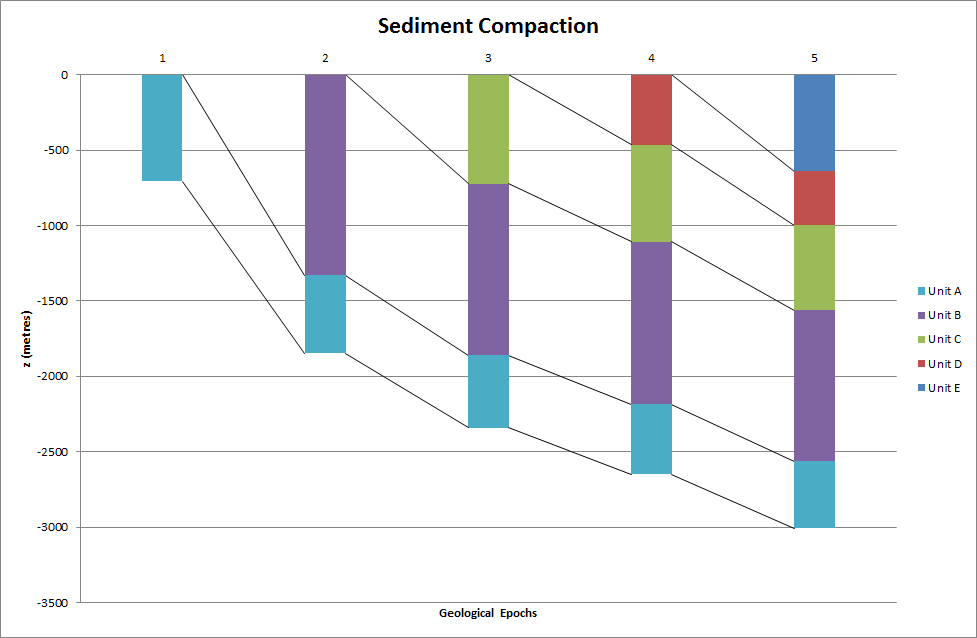
\includegraphics[width=0.9\linewidth]{fig-models/Compaction_of_Sediment.png}}
  \caption{
  Illustration of the compaction of geological layers (with different colors) through time. \label{decay:app:sediment:fig:layers}
  }
\end{figure}
%\clearpage % flush figures decay:app:sediment:fig:layers


When we drill a well at present time through the right-most column of
sediments in Figure~\ref{decay:app:sediment:fig:layers}, we can measure
the thickness of the sediment in (say) the bottom layer. Let $L_1$ be
this thickness.  Assuming that the volume of sediment remains constant
through time, we have that the initial volume, $\int_0^{L_{1,0}}
\phi_1 dz$, must equal the volume seen today,
$\int_{\ell-L_1}^{\ell}\phi_1 dz$, where $\ell$ is the depth of the
bottom of the sediment in the present day configuration.  After having
solved for $\phi_1$ as a function of $z$, we can then find the
original thickness $L_{1,0}$ of the sediment from the equation

\[ \int_0^{L_{1,0}} \phi_1 dz = \int_{\ell-L_1}^{\ell}\phi_1 dz \tp \]
In hydrocarbon exploration it is important to know $L_{1,0}$ and the
compaction history of the various layers of sediments.

\section{Vertical motion of a body in a viscous fluid}
\label{decay:app:drag}


A body moving vertically through a fluid (liquid or gas) is subject to
three different types of forces: the gravity force, \href{{http://en.wikipedia.org/wiki/Drag_(physics)}}{the drag force},
and the buoyancy force.

\subsection{Overview of forces}

Taking the upward direction as positive,
the gravity force is $F_g= -mg$, where $m$ is the mass of the body and
$g$ is the acceleration of gravity.
The uplift or buoyancy force (``Archimedes force'') is $F_b = \varrho gV$,
where $\varrho$ is the density of the fluid and
$V$ is the volume of the body.

The drag force is of two types, depending on the Reynolds number
\begin{equation}
\hbox{Re} = \frac{\varrho d|v|}{\mu},
\end{equation}
where $d$ is the diameter of the body in
the direction perpendicular to the flow, $v$ is the velocity of the
body, and $\mu$ is the dynamic viscosity of the fluid.
When $\hbox{Re} < 1$, the drag force is fairly well modeled by
the so-called Stokes' drag,
which for a spherical body of diameter $d$ reads
\begin{equation}
F_d^{(S)} = - 3\pi d\mu v
\tp
\end{equation}
Quantities are taken as positive in the upwards vertical direction, so
if $v>0$ and the body moves upwards, the drag force acts downwards and
become negative, in accordance with the minus sign in expression for
$F_d^{(S)}$.

For large Re, typically $\hbox{Re} > 10^3$, the drag force is quadratic
in the velocity:
\begin{equation}
F_d^{(q)} = -{1\over2}C_D\varrho A|v|v,
\end{equation}
where $C_D$ is a dimensionless drag coefficient depending on the body's shape,
and $A$ is the cross-sectional area as
produced by a cut plane, perpendicular to the motion, through the thickest
part of the body. The superscripts $\,{}^q$ and $\,{}^S$ in
$F_d^{(S)}$ and $F_d^{(q)}$ indicate Stokes drag and quadratic drag,
respectively.

\subsection{Equation of motion}

All the mentioned forces act in the vertical direction.
Newton's second law of motion applied to the body says that the sum of
these forces must equal the mass of the body times its acceleration
$a$ in the vertical direction.

\begin{equation*} ma = F_g + F_d^{(S)} + F_b \tp\end{equation*}
Here we have chosen to model the fluid resistance by the Stokes drag.
Inserting the expressions for the forces yields

\[  ma = -mg - 3\pi d\mu v + \varrho gV
\tp
\]
The unknowns here are $v$ and $a$, i.e., we have two unknowns but only
one equation. From kinematics in physics we know that
the acceleration is the time derivative of the velocity: $a = dv/dt$.
This is our second equation.
We can easily eliminate $a$ and get a single differential equation for $v$:

\[ m{dv\over dt} = -mg - 3\pi d\mu v + \varrho gV
\tp
\]
A small rewrite of this equation is handy: We express $m$ as $\varrho_bV$,
where $\varrho_b$ is the density of the body, and we divide by
the mass to get

\begin{equation}
v^{\prime}(t) = - \frac{3\pi d\mu}{\varrho_b V} v + g\left(\frac{\varrho}{\varrho_b} -1\right)
\label{decay:app:fallingbody:model:S}
\tp
\end{equation}
We may introduce the constants
\begin{equation}
a = \frac{3\pi d\mu}{\varrho_b V},\quad
b = g\left(\frac{\varrho}{\varrho_b} -1\right),
\end{equation}
so that the structure of the differential equation becomes obvious:

\begin{equation}
v^{\prime}(t) = -av(t) + b
\label{decay:app:fallingbody:gmodel:S}
\tp
\end{equation}
The corresponding initial condition is $v(0)=v_0$ for some prescribed
starting velocity $v_0$.

This derivation can be repeated with the quadratic drag force
$F_d^{(q)}$, leading to the result

\begin{equation}
v^{\prime}(t) =
-{1\over2}C_D{\varrho A\over\varrho_b V}|v|v +
g\left({\varrho\over\varrho_b} - 1\right)
\tp
\label{decay:app:fallingbody:model:q}
\end{equation}
Defining

\begin{equation}
a = {1\over2}C_D{\varrho A\over\varrho_b V},
\end{equation}
and $b$ as above, we can write (\ref{decay:app:fallingbody:model:q}) as
\begin{equation}
v^{\prime}(t) = -a|v|v + b
\tp
\label{decay:app:fallingbody:gmodel:q}
\end{equation}

\index{terminal velocity}

\subsection{Terminal velocity}

An interesting aspect of (\ref{decay:app:fallingbody:gmodel:S}) and
(\ref{decay:app:fallingbody:gmodel:q}) is whether $v$ will approach
a final constant value,
the so-called \emph{terminal velocity} $v_T$, as $t\rightarrow\infty$.
A constant $v$ means that
$v^{\prime}(t)\rightarrow 0$ as $t\rightarrow\infty$ and therefore
the terminal velocity $v_T$ solves

\[ 0 = -av_T + b \]
and
\[ 0 = -a|v_T|v_T + b\tp \]
The former equation implies $v_T = b/a$, while the latter has solutions
$v_T =-\sqrt{|b|/a}$ for a falling body ($v_T < 0$) and
$v_T = \sqrt{b/a}$ for a rising body ($v_T>0$).

\subsection{A Crank-Nicolson scheme}

Both governing equations, the Stokes' drag model
(\ref{decay:app:fallingbody:gmodel:S}) and the quadratic drag model
(\ref{decay:app:fallingbody:gmodel:q}), can be readily solved
by the Forward Euler scheme. For higher accuracy one can use
the Crank-Nicolson method, but a straightforward application
of this method gives
a nonlinear equation in the new unknown value $v^{n+1}$ when applied to
(\ref{decay:app:fallingbody:gmodel:q}):

\begin{equation}
\frac{v^{n+1}-v^n}{\Delta t}
= -a\half(|v^{n+1}|v^{n+1} + |v^n|v^n) + b
\label{decay:app:fallingbody:gmodel:CN}
\tp
\end{equation}
The first term on the right-hand side of (\ref{decay:app:fallingbody:gmodel:CN})
is the arithmetic average of $-|v|v$ evaluated at time levels $n$ and $n+1$.

Instead of approximating the term $-|v|v$ by an arithmetic
average, we can use a \emph{geometric mean}:

\index{geometric mean}
\index{averaging!geometric}

\begin{equation}
(|v|v)^{n+\half} \approx |v^n|v^{n+1}
\tp
\end{equation}
The error is of second order in $\Delta t$, just as for the arithmetic
average and the centered finite difference approximation in
(\ref{decay:app:fallingbody:gmodel:CN}). With the geometric mean,
the resulting discrete equation

\[
\frac{v^{n+1}-v^n}{\Delta t} = - a|v^{n}|v^{n+1} + b
\]
becomes a \emph{linear} equation in $v^{n+1}$, and we can
therefore easily solve for $v^{n+1}$:

\begin{equation}
v^{n+1} = \frac{v_n + \Delta t b^{n+\half}}{1 + \Delta t a^{n+\half}|v^{n}|}\tp
\label{decay:app:fallingbody:gmodel:q:CN}
\end{equation}

Using a geometric mean instead of an arithmetic mean in the Crank-Nicolson
scheme is an attractive method for avoiding a nonlinear algebraic
equation when discretizing a nonlinear ODE.

% Is the error actually of second order for an arbitrary a(u)u term?

\subsection{Physical data}

Suitable values of $\mu$ are $1.8\cdot 10^{-5}\hbox{ Pa}\, \hbox{s}$ for air
and $8.9\cdot 10^{-4}\hbox{ Pa}\, \hbox{s}$ for water.
Densities can be taken as $1.2\hbox{ kg/m}^3$ for air and as
$1.0\cdot 10^3\hbox{ kg/m}^3$ for water. For considerable vertical
displacement in the atmosphere one should take into account that
the density of air varies with the altitude, see Section~\ref{decay:app:atm}.
One possible density variation arises from the one-layer model
in the mentioned section.

Any density variation makes $b$ time dependent and we need
$b^{n+\half}$ in (\ref{decay:app:fallingbody:gmodel:q:CN}).
To compute the density that enters
$b^{n+\half}$ we must also compute the vertical
position $z(t)$ of the body. Since $v=dz/dt$, we can use a centered
difference approximation:

\[ \frac{z^{n+\half} - z^{n-\half}}{\Delta t} = v^n
\quad\Rightarrow\quad z^{n+\half} = z^{n-\half}+\Delta t\, v^n\tp\]
This $z^{n+\half}$ is used in the expression for $b$
to compute $\varrho(z^{n+\half})$ and then $b^{n+\half}$.

The \href{{http://en.wikipedia.org/wiki/Drag_coefficient}}{drag coefficient} $C_D$ depends heavily
on the shape of the body.  Some values are: 0.45 for a sphere, 0.42
for a semi-sphere, 1.05 for a cube, 0.82 for a long cylinder (when the
center axis is in the vertical direction), 0.75 for a rocket,
1.0-1.3 for a man in upright position, 1.3 for a flat plate perpendicular
to the flow, and
0.04 for a streamlined, droplet-like body.

\subsection{Verification}

To verify the program, one may assume a heavy body in air such that the $F_b$
force can be neglected, and further assume a small velocity such that the
air resistance $F_d$ can also be neglected. This can be obtained by
setting $\mu$ and $\varrho$ to zero. The motion then leads to
the velocity
$v(t)=v_0 - gt$, which is linear in $t$ and therefore should be
reproduced to machine precision (say tolerance $10^{-15}$) by any
implementation based on the Crank-Nicolson or Forward Euler schemes.

Another verification, but not as powerful as the one above,
can be based on computing the terminal velocity and comparing with
the exact expressions.
The advantage of this verification is that we can also
test the situation $\varrho\neq 0$.

As always, the method of manufactured solutions can be applied to
test the implementation of all terms in the governing equation, but
then the solution has no physical relevance in general.

\index{scaling}

\subsection{Scaling}
\label{decay:app:drag:scaling}

Applying scaling, as described in Section~\ref{decay:app:scaling},
will for the linear case reduce the need to estimate values for
seven parameters down to choosing one value of a single dimensionless parameter

\[ \beta = \frac{\varrho_b gV\left(\frac{\varrho}{\varrho_b} -1\right)}{3\pi d\mu I},\]
provided $I\neq 0$. If the motion starts from rest, $I=0$, the scaled
problem reads

\[ \bar u^{\prime}=1-\bar u, \quad \bar u(0)=0,\]
and there is
no need for estimating physical parameters (!).
This means that there is a single universal solution to the problem
of a falling body starting from rest:
$\bar u(t) = 1 - e^{-\bar t}$. All real
physical cases correspond to stretching the $\bar t$ axis and the $\bar u$
axis in this dimensionless solution. More precisely, the physical velocity
$u(t)$ is related to the dimensionless velocity $\bar u(\bar t)$ through

\[ u = \frac{\varrho_bgV\left(\frac{\varrho}{\varrho_b} -1\right)}{3\pi d\mu}\bar u(t/(g(\varrho/\varrho_b -1))) =
\frac{\varrho_bgV\left(\frac{\varrho}{\varrho_b} -1\right)}{3\pi d\mu}(1 -
e^{t/(g(\varrho/\varrho_b -1))})\tp\]

\section{Viscoelastic materials}
\label{decay:app:viscoelasticity}

\index{Kelvin-Voigt material model}
\index{viscoelasticity}

When stretching a rod made of a perfectly elastic material, the
elongation (change in the rod's
length) is proportional to the magnitude of the applied force.
Mathematical models for material behavior under application of
external forces use \emph{strain} $\varepsilon$
and \emph{stress} $\sigma$ instead of elongation and
forces. Strain is relative change in elongation and stress is force
per unit area. An elastic material has a linear relation between
stress and strain:  $\sigma = E\varepsilon$. This is a good model
for many materials, but frequently the velocity of the deformation
(or more precisely, the strain rate $\varepsilon^{\prime}$)
also influences the stress. This is particularly the case for
materials like organic polymers, rubber, and wood. When the stress
depends on both the strain and the strain rate, the material is
said to be viscoelastic. A common model relating forces to deformation
is the \href{{https://en.wikipedia.org/wiki/Kelvin-Voigt_material}}{Kelvin-Voigt model}:

\begin{equation}
\sigma(t) = E\varepsilon(t) + \eta\varepsilon^{\prime}(t)\tp
\label{decay:app:viscoelasticity:se}
\end{equation}
Compared to a perfectly elastic material, which deforms instantaneously
when a force is acting, a Kelvin-Voigt material will spend some time
to elongate. For example, when an elastic rod is subject to a constant
force $\stress$ at $t=0$, the strain immediately adjusts to $\varepsilon
=\sigma/E$. A Kelvin-Voigt material, however, has a response
$\varepsilon(t) = \frac{\sigma}{E}(1-e^{Et/\eta})$. Removing the force
when the strain is $\varepsilon(t_1) = I$ will for an elastic material
immediately bring the strain back to zero, while a Kelvin-Voigt
material will decay: $\varepsilon = Ie^{-(t-t_1)E/\eta)}$.

Introducing $u$ for $\varepsilon$ and treating $\stress(t)$ as a
given function, we can write the Kelvin-Voigt model in our standard form

\begin{equation}
u^{\prime}(t) = -au(t) + b(t),
\end{equation}
with $a = E/\eta$ and $b(t)=\stress(t)/\eta$. An initial condition,
usually $u(0)=0$, is needed.




\section{Decay ODEs from solving a PDE by Fourier expansions}
\label{decay:app:diffusion:Fourier}

% Maybe move to diffusion part? Makes sense there too, or refer...or
% repeat, or make one exer with two k's and then generalize in diffusion

Suppose we have a partial differential equation
\[ \frac{\partial u}{\partial t} = \alpha\frac{\partial^2u}{\partial x^2}
+ f(x,t),
\]
with boundary conditions $u(0,t)=u(L,t)=0$ and initial condition
$u(x,0)=I(x)$. One may express the solution as
\[ u(x,t) = \sum_{k=1}^m A_k(t)e^{ikx\pi/L},\]
for appropriate unknown functions $A_k$, $k=1,\ldots,m$.
We use the complex exponential $e^{ikx\pi/L}$ for easy algebra, but
the physical $u$ is taken as the real part of any complex expression.
Note that the expansion in terms of $e^{ikx\pi/L}$ is compatible with
the boundary conditions: all functions $e^{ikx\pi/L}$ vanish for
$x=0$ and $x=L$. Suppose we can express $I(x)$ as

\[ I(x) = \sum_{k=1}^m I_ke^{ikx\pi/L}
\tp
\]
Such an expansion can be computed by well-known Fourier expansion techniques,
but those details are not important here.
Also, suppose we can express the given $f(x,t)$ as
\[ f(x,t) = \sum_{k=1}^m b_k(t)e^{ikx\pi/L}
\tp
\]
Inserting the expansions for $u$
and $f$ in the differential equations demands that all terms corresponding
to a given $k$ must be equal. The calculations result in the follow
system of ODEs:

\[
A_k^{\prime}(t) = -\alpha\frac{k^2\pi^2}{L^2} + b_k(t),\quad k=1,\ldots,m
\tp
\]
From the initial condition
\[ u(x,0)=\sum_k A_k(0)e^{ikx\pi/L}=I(x)=\sum_k I_k e^{(ikx\pi/L)},\]
so it follows that $A_k(0)=I_k$, $k=1,\ldots,m$. We then have $m$
equations of the form $A_k^{\prime}=-a A_k +b$, $A_k(0)=I_k$, for
appropriate definitions of $a$ and $b$. These ODE problems
are independent of each other such that we can solve one problem
at a time. The outlined technique is a quite common solution approach to
partial differential equations.

\paragraph{Remark.}
Since $a_k$ depends on $k$ and the stability of the
Forward Euler scheme demands $a_k\Delta t \leq 1$, we get that $\Delta
t \leq \alpha^{-1}L^2\pi^{-2} k^{-2}$ for this scheme.  Usually, quite
large $k$ values are needed to accurately represent the given
functions $I$ and $f$ so that $\Delta t$ in the Forward Euler scheme
needs to be very small for these large values of $k$.  Therefore, the
Crank-Nicolson and Backward Euler schemes, which allow larger $\Delta
t$ without any growth in the solutions, are more popular choices when
creating time-stepping algorithms for partial differential equations
of the type considered in this example.


\section{Exercises}



% --- begin exercise ---
\begin{doconceexercise}
\refstepcounter{doconceexercisecounter}

\subsection*{Problem \thedoconceexercisecounter: Radioactive decay of Carbon-14}

\label{decay:app:exer:radio:C14}

The \href{{http://en.wikipedia.org/wiki/Carbon-14}}{Carbon-14} isotope,
whose radioactive decay is used extensively in dating organic material
that is tens of thousands of years old, has a half-life of $5,730$
years.  Determine the age of an organic material that contains 8.4 percent
of its initial amount of Carbon-14.  Use a time unit of 1 year in the
computations.  The uncertainty in the half time of Carbon-14 is $\pm
40$ years.  What is the corresponding uncertainty in the estimate of
the age?

% --- begin hint in exercise ---

\paragraph{Hint 1.}
Let $A$ be the amount of Carbon-14. The ODE problem is then
$A^{\prime}(t)=-aA(t)$, $A(0)=I$. Introduced the scaled amount
$u=A/I$. The ODE problem for $u$ is $u^{\prime}=-au$, $u(0)=1$.
Measure time in years.
Simulate until the first mesh point $t_m$ such that $u(t_m)\leq 0.084$.

% --- end hint in exercise ---

% --- begin hint in exercise ---

\paragraph{Hint 2.}
Use simulations with $5,730\pm 40$ y as input
and find the corresponding uncertainty interval for the result.

% --- end hint in exercise ---


% removed !bsol ... !esol environment (because of the command-line option --without_solutions)
\noindent Filename: \texttt{carbon14}.

\end{doconceexercise}
% --- end exercise ---




% --- begin exercise ---
\begin{doconceexercise}
\refstepcounter{doconceexercisecounter}

\subsection*{Exercise \thedoconceexercisecounter: Derive schemes for Newton's law of cooling}

\label{decay:app:exer:cooling:schemes}

Show in detail how we can apply the ideas of the Forward Euler,
Backward Euler, and Crank-Nicolson
discretizations to derive explicit
computational formulas for new temperature values in Newton's law of
cooling (see Section~\ref{decay:app:Newton:cooling}):

\[
\frac{dT}{dt} = -k(T-T_s(t)),\quad T(0)=T_0\tp
\]
Here, $T$ is the temperature of the body, $T_s(t)$ is the temperature
of the surroundings, $t$ is time, $k$ is the heat transfer
coefficient, and $T_0$ is the initial temperature of the body.
Summarize the discretizations in a $\theta$-rule
such that you can get the three
schemes from a single formula by varying the $\theta$ parameter.


% removed !bsol ... !esol environment (because of the command-line option --without_solutions)
\noindent Filename: \Verb!schemes_cooling!.

\end{doconceexercise}
% --- end exercise ---




% --- begin exercise ---
\begin{doconceexercise}
\refstepcounter{doconceexercisecounter}

\subsection*{Exercise \thedoconceexercisecounter: Implement schemes for Newton's law of cooling}

\label{decay:app:exer:cooling:py}

The goal of this exercise is to implement the schemes from
Exercise~\ref{decay:app:exer:cooling:schemes} and investigate
several approaches for verifying the implementation.


\subex{a)}
Implement the $\theta$-rule from
Exercise~\ref{decay:app:exer:cooling:schemes} in a function

\begin{cod}{cbg_blue1}\begin{Verbatim}[numbers=none,fontsize=\fontsize{9pt}{9pt},baselinestretch=0.95,xleftmargin=2mm]
cooling(T0, k, T_s, t_end, dt, theta=0.5)
\end{Verbatim}
\end{cod}
\noindent
where \texttt{T0} is the initial temperature, \texttt{k} is
the heat transfer coefficient, \Verb!T_s! is a function of \texttt{t} for
the temperature of the
surroundings, \Verb!t_end! is the end time of the simulation, \texttt{dt} is the
time step, and \texttt{theta} corresponds to $\theta$.  The \texttt{cooling}
function should return the temperature as an array \texttt{T} of values at
the mesh points and the time mesh \texttt{t}.


% removed !bsol ... !esol environment (because of the command-line option --without_solutions)

\subex{b)}
In the case $\lim_{t\rightarrow\infty}T_s(t)=C=\mbox{const}$,
explain why $T(t)\rightarrow C$. Construct an example where you
can illustrate this property in a plot. Implement a corresponding
test function that checks the correctness of the asymptotic
value of the solution.


% removed !bsol ... !esol environment (because of the command-line option --without_solutions)

\subex{c)}
A piecewise constant surrounding temperature,

\[ T_s(t) = \left\lbrace\begin{array}{ll} C_0,& 0\leq t\leq t^*\\ 
C_1, & t>t^*,\end{array}\right.
\]
corresponds to a sudden change in the environment
at $t=t^*$. Choose $C_0=2T_0$, $C_1=\frac{1}{2}T_0$, and
$t^*=3/k$. Plot the solution $T(t)$ and explain why it seems physically
reasonable.


% removed !bsol ... !esol environment (because of the command-line option --without_solutions)

\subex{d)}
We know from the ODE $u^\prime =-au$ that the Crank-Nicolson scheme
can give non-physical oscillations for $\Delta t > 2/a$.
In the present problem, this results indicates
that the Crank-Nicolson scheme give undesired
oscillations for $\Delta t > 2/k$.
Discuss if this a potential problem in the physical case from c).


% removed !bsol ... !esol environment (because of the command-line option --without_solutions)

\subex{e)}
Find an expression for the exact solution of
$T^{\prime} = -k(T-T_s(t))$, $T(0)=T_0$.
Construct a test case and compare the
numerical and exact solution in a plot.

Find a value of the time step
$\Delta t$ such that the two solution curves cannot (visually) be
distinguished from each other. Many scientists will claim that such a
plot provides evidence for a correct implementation, but point out why
there still may be errors in the code.  Can you introduce bugs in the
\texttt{cooling} function and still achieve visually coinciding curves?

% --- begin hint in exercise ---

\paragraph{Hint.}
The exact solution can be derived by multiplying (\ref{decay:Newton:cooling})
by the integrating factor $e^{kt}$.

% --- end hint in exercise ---


% removed !bsol ... !esol environment (because of the command-line option --without_solutions)

\subex{f)}
Implement a test function for checking that the solution returned by
the \texttt{cooling} function is identical to the exact numerical
solution of the problem (to machine precision) when $T_s$ is constant.

% --- begin hint in exercise ---

\paragraph{Hint.}
The exact solution of the
discrete equations in the case $T_s$ is a constant can be found by
introducing $u=T-T_s$ to get a problem $u^{\prime}=-ku$, $u(0)=T_0-T_s$.
The solution of the discrete equations is then of the form
$u^{n}=(T_0-T_s)A^n$ for some amplification factor $A$. The
expression for $T^n$ is then $T^n = T_s(t_n) + u^n =
T_s + (T_0-T_s)A^n$.
We find that

\[ A = \frac{1 - (1-\theta) k\Delta t}{1 + \theta k\Delta t}\tp\]
The test function, testing several $\theta$ values for a quite coarse
mesh, may take the form

\begin{cod}{cbg_blue1}\begin{Verbatim}[numbers=none,fontsize=\fontsize{9pt}{9pt},baselinestretch=0.95,xleftmargin=2mm]
def test_discrete_solution():
    """
    Compare the numerical solution with an exact solution of the scheme
    when the T_s is constant.
    """
    T_s = 10
    T0 = 2
    k = 1.2
    dt = 0.1   # can use any mesh
    N_t = 6    # any no of steps will do
    t_end = dt*N_t
    t = np.linspace(0, t_end, N_t+1)

    for theta in [0, 0.5, 1, 0.2]:
        u, t = cooling(T0, k, lambda t: T_s , t_end, dt, theta)
        A = (1 - (1-theta)*k*dt)/(1 + theta*k*dt)
        u_discrete_exact = T_s + (T0-T_s)*A**(np.arange(len(t)))
        diff = np.abs(u - u_discrete_exact).max()
        print 'diff computed and exact discrete solution:', diff
        tol = 1E-14
        success = diff < tol
        assert success, 'diff=%g' % diff
\end{Verbatim}
\end{cod}
\noindent
Running this function shows that the \texttt{diff} variable is \texttt{3.55E-15}
as maximum so a tolerance of $10^{-14}$ is appropriate.
This is a good test that the \texttt{cooling} function works!

% --- end hint in exercise ---

\noindent Filename: \texttt{cooling}.

\end{doconceexercise}
% --- end exercise ---




% --- begin exercise ---
\begin{doconceexercise}
\refstepcounter{doconceexercisecounter}

\subsection*{Exercise \thedoconceexercisecounter: Find time of murder from body temperature}

\label{decay:app:exer:cooling:murder}

% \href{{http://www.biology.arizona.edu/BioMath/tutorials/Applications/Cooling.html}}{\nolinkurl{http://www.biology.arizona.edu/BioMath/tutorials/Applications/Cooling.html}}

A detective measures the temperature of a dead body to be 26.7 C at 2
pm. One hour later the temperature is 25.8 C. The question is when
death occurred.

Assume that Newton's law of cooling (\ref{decay:Newton:cooling}) is an
appropriate mathematical model for the evolution of the temperature in
the body.  First, determine $k$ in (\ref{decay:Newton:cooling}) by
formulating a Forward Euler approximation with one time steep from
time 2 am to time 3 am, where knowing the two temperatures allows for
finding $k$. Assume the temperature in the air to be 20 C. Thereafter,
simulate the temperature evolution from the time of murder, taken as
$t=0$, when $T=37\hbox{ C}$, until the temperature reaches 25.8 C. The
corresponding time allows for answering when death occurred.


% removed !bsol ... !esol environment (because of the command-line option --without_solutions)
\noindent Filename: \texttt{detective}.

\end{doconceexercise}
% --- end exercise ---




% --- begin exercise ---
\begin{doconceexercise}
\refstepcounter{doconceexercisecounter}

\subsection*{Exercise \thedoconceexercisecounter: Simulate an oscillating cooling process}

\label{decay:app:exer:cooling:osc}

The surrounding temperature $T_s$ in Newton's law of cooling
(\ref{decay:Newton:cooling}) may vary in time. Assume that the
variations are periodic with period $P$ and amplitude $a$ around
a constant mean temperature $T_m$:

\begin{equation}
T_s(t) = T_m + a\sin\left(\frac{2\pi}{P}t\right)
\tp
\end{equation}
Simulate a process with the following data: $k=0.05 \hbox{ min}^{-1}$,
$T(0)=5$ C, $T_m=25$ C, $a=2.5$ C, and $P=1$ h, $P=10$ min, and $P=6$ h.
Plot the $T$ solutions and $T_s$ in the same plot.


% removed !bsol ... !esol environment (because of the command-line option --without_solutions)
\noindent Filename: \Verb!osc_cooling!.

\end{doconceexercise}
% --- end exercise ---




% --- begin exercise ---
\begin{doconceexercise}
\refstepcounter{doconceexercisecounter}

\subsection*{Exercise \thedoconceexercisecounter: Simulate stochastic radioactive decay}

\label{decay:app:exer:stoch:nuclear}

The purpose of this exercise is to implement the stochastic model
described in Section~\ref{decay:app:nuclear} and show that its
mean behavior approximates the solution of the corresponding
ODE model.

The simulation goes on for a time interval $[0,T]$ divided into
$N_t$ intervals of length $\Delta t$. We start with $N_0$
atoms. In some time interval, we have $N$ atoms that have survived.
Simulate $N$ Bernoulli trials with probability $\lambda\Delta t$
in this interval by drawing $N$ random numbers, each being 0 (survival)
or 1 (decay), where the probability of getting 1 is $\lambda\Delta t$.
We are interested in the number of decays, $d$, and the number of
survived atoms in the next interval is then $N-d$.
The Bernoulli trials
are simulated by drawing $N$ uniformly distributed real numbers on
$[0,1]$ and saying that 1 corresponds to a value less than $\lambda\Delta t$:

\begin{cod}{cbg_blue1}\begin{Verbatim}[numbers=none,fontsize=\fontsize{9pt}{9pt},baselinestretch=0.95,xleftmargin=2mm]
# Given lambda_, dt, N
import numpy as np
uniform = np.random.uniform(N)
Bernoulli_trials = np.asarray(uniform < lambda_*dt, dtype=np.int)
d = Bernoulli_trials.size
\end{Verbatim}
\end{cod}
\noindent
Observe that \Verb!uniform < lambda_*dt! is a boolean array whose true
and false values become 1 and 0, respectively, when converted to an
integer array.

Repeat the simulation over $[0,T]$ a large number of times, compute the average
value of $N$ in each interval, and compare with the solution of
the corresponding ODE model.
\noindent Filename: \Verb!stochastic_decay!.

\end{doconceexercise}
% --- end exercise ---




% --- begin exercise ---
\begin{doconceexercise}
\refstepcounter{doconceexercisecounter}

\subsection*{Problem \thedoconceexercisecounter: Radioactive decay of two substances}

\label{decay:app:exer:radio:twosubst}

Consider two radioactive substances A and B. The nuclei in substance A
decay to form nuclei of type B with a half-life $A_{1/2}$, while
substance B decay to form type A nuclei with a half-life $B_{1/2}$.
Letting $u_A$ and $u_B$ be the fractions of the initial amount of
material in substance A and B, respectively, the following system of
ODEs governs the evolution of $u_A(t)$ and $u_B(t)$:
\begin{align}
\frac{1}{\ln 2} u_A^{\prime} &= u_B/B_{1/2} - u_A/A_{1/2},\\ 
\frac{1}{\ln 2} u_B^{\prime} &= u_A/A_{1/2} - u_B/B_{1/2},
\end{align}
with $u_A(0)=u_B(0)=1$.


\subex{a)}
Make a simulation program that solves for $u_A(t)$ and $u_B(t)$.

\subex{b)}
Verify the implementation by computing analytically
the limiting values of
$u_A$ and $u_B$ as $t\rightarrow \infty$ (assume $u_A^{\prime},u_B^{\prime}\rightarrow 0$)
and comparing these with those obtained numerically.

\subex{c)}
Run the program for the case of $A_{1/2}=10$ minutes and $B_{1/2}=50$ minutes.
Use a time unit of 1 minute. Plot $u_A$ and $u_B$ versus time in the same
plot.

\noindent Filename: \Verb!radioactive_decay_2subst!.

\end{doconceexercise}
% --- end exercise ---




% --- begin exercise ---
\begin{doconceexercise}
\refstepcounter{doconceexercisecounter}

\subsection*{Exercise \thedoconceexercisecounter: Simulate a simple chemical reaction}

\label{decay:app:exer:kinetics:AB}

Consider the simple chemical reaction where a substance A is turned
into a substance B according to

\begin{align*}
\frac{d[A]}{dt} &= -k[A],\\ 
\frac{d[B]}{dt} &= k[A],\\ 
\end{align*}
where $[A]$ and $[B]$ are the concentrations of A and B, respectively.
It may be a challenge to find appropriate values of $k$, but we can avoid
this problem by working with a scaled model (as explained in
Section~\ref{decay:app:scaling}).
Scale the model above, using a time scale $1/k$, and use
the initial concentration
of $[A]$ as scale for $[A]$ and $[B]$. Show that the scaled system
reads

\begin{align*}
\frac{du}{dt} &= -u,\\ 
\frac{dv}{dt} &= u,\\ 
\end{align*}
with initial conditions $u(0)=1$, and $v(0)=\alpha$, where
$\alpha = [B](0)/[A](0)$ is a dimensionless number, and
$u$ and $v$ are the scaled concentrations of $[A]$ and $[B]$,
respectively. Implement a numerical scheme that can be used to
find the solutions
$u(t)$ and $v(t)$. Visualize $u$ and $v$ in the same plot.
\noindent Filename: \Verb!chemcial_kinetics_AB!.

\end{doconceexercise}
% --- end exercise ---




% --- begin exercise ---
\begin{doconceexercise}
\refstepcounter{doconceexercisecounter}

\subsection*{Exercise \thedoconceexercisecounter: Simulate an $n$-th order chemical reaction}

\label{decay:app:exer:kinetics:ABn}

An $n$-order chemical reaction, generalizing the model in
Exercise~\ref{decay:app:exer:kinetics:AB}, takes the form

\begin{align*}
\frac{d[A]}{dt} &= -k[A]^n,\\ 
\frac{d[B]}{dt} &= k[A]^n,\\ 
\end{align*}
where symbols are as defined in Exercise~\ref{decay:app:exer:kinetics:AB}.
Bring this model on dimensionless form, using a time scale $[A](0)^{n-1}/k$,
and show that the dimensionless model simplifies to

\begin{align*}
\frac{du}{dt} &= -u^n,\\ 
\frac{dv}{dt} &= u^n,\\ 
\end{align*}
with $u(0)=1$ and $v(0)=\alpha = [B](0)/[A](0)$. Solve numerically for
$u(t)$ and show a plot with $u$ for $n=0.5, 1, 2, 4$.
\noindent Filename: \Verb!chemcial_kinetics_ABn!.

\end{doconceexercise}
% --- end exercise ---




% --- begin exercise ---
\begin{doconceexercise}
\refstepcounter{doconceexercisecounter}

\subsection*{Exercise \thedoconceexercisecounter: Simulate a biochemical process}

\label{decay:app:exer:MMK}

The purpose of this exercise is to simulate the ODE system
(\ref{decay:app:MMK:ES1})-(\ref{decay:app:MMK:E1}) modeling a simple
biochemical process.


\subex{a)}
Scale (\ref{decay:app:MMK:ES1})-(\ref{decay:app:MMK:E1}) such that
we can work with dimensionless parameters, which are easier to prescribe.
Introduce

\[ \bar Q = \frac{[ES]}{Q_c},\quad
\bar P = \frac{P}{P_c},\quad \bar S = \frac{S}{S_0},\quad \bar E = \frac{E}{E_0},\quad \bar t = \frac{t}{t_c},\]
where appropriate scales are

\[ Q_c = \frac{S_0E_0}{K},\quad P_c = Q_c, \quad t_c=\frac{1}{k_+E_0},\]
with $K=(k_v+k_-)/k_+$ (Michaelis constant). Show that the scaled
system becomes

\begin{align}
\frac{d\bar Q}{d\bar t} &= \alpha (\bar E\bar S
- \bar Q),
\label{decay:app:MMK:Q2}\\ 
\frac{d\bar P}{d\bar t} &= \beta\bar Q,
\label{decay:app:MMK:P2}\\ 
\frac{d\bar S}{d\bar t} &= -\bar E\bar S
+ (1 - \beta\alpha^{-1})\bar Q,
\label{decay:app:MMK:S2}\\ 
\epsilon\frac{d\bar E}{d\bar t} &= -\bar E\bar S + \bar Q,
\label{decay:app:MMK:E2}
\end{align}
where we have three dimensionless parameters

\[ \alpha = \frac{K}{E_0},\quad \beta = \frac{k_v}{k_+ E_0},\quad
\epsilon = \frac{E_0}{S_0}\tp
\]
The corresponding initial conditions are $\bar Q=\bar P=0$ and
$\bar S=\bar E=1$.


% removed !bsol ... !esol environment (because of the command-line option --without_solutions)

\subex{b)}
Implement a function for
solving (\ref{decay:app:MMK:Q2})-(\ref{decay:app:MMK:E2}).


% removed !bsol ... !esol environment (because of the command-line option --without_solutions)

\subex{c)}
There are two conservation equations implied by
(\ref{decay:app:MMK:ES1})-(\ref{decay:app:MMK:E1}):

\begin{align}
[ES] + [E] &= E_0,\\ 
[ES] + [S] + [P] &= S_0\tp
\end{align}
Derive these two equations. Use these properties in the function
in b) to do a partial verification of the solution at each time step.


% removed !bsol ... !esol environment (because of the command-line option --without_solutions)

\subex{d)}
Simulate a case with $T=8$, $\alpha = 1$, $\beta=4$, and two
$\epsilon$ values: 0.9 and 0.1.


% removed !bsol ... !esol environment (because of the command-line option --without_solutions)

\noindent Filename: \texttt{biochem}.

\end{doconceexercise}
% --- end exercise ---




% --- begin exercise ---
\begin{doconceexercise}
\refstepcounter{doconceexercisecounter}

\subsection*{Exercise \thedoconceexercisecounter: Simulate spreading of a disease}

\label{decay:app:exer:SIR}

The SIR model (\ref{decay:app:SIR:S})-(\ref{decay:app:SIR:R}) can be used
to simulate spreading of an epidemic disease.


\subex{a)}
Estimating the parameter $\beta$
is difficult so it can be handy to scale the equations. Use
$t_c=1/\nu$ as time scale, and scale $S$, $I$, and $R$ by
the population size $N=S(0)+I(0)+R(0)$. Show that the resulting dimensionless
model becomes

\begin{align}
\frac{d\bar S}{d\bar t} &= - R_0\bar S\bar I,
\label{decay:app:SIR:S2}\\ 
\frac{d\bar I}{d\bar t} &= R_0 \bar S\bar I - \bar I,
\label{decay:app:SIR:I2}\\ 
\frac{d\bar R}{d\bar t} &= I,
\label{decay:SIR:R2}\\ 
\bar S(0) &= 1-\alpha,\\ 
\bar I(0) &= \alpha,\\ 
\bar R(0) &= 0,
\end{align}
where $R_0$ and $\alpha$ are the only parameters in the problem:

\[ R_0 = \frac{N\beta}{\nu}, \quad \alpha = \frac{I(0)}{N}\tp\]
A quantity with a bar denotes a dimensionless version of that quantity, e.g,
$\bar t$ is dimensionless time, and $\bar t = \nu t$.


% removed !bsol ... !esol environment (because of the command-line option --without_solutions)

\subex{b)}
Show that the $R_0$ parameter governs whether the disease will spread
or not at $t=0$.

% --- begin hint in exercise ---

\paragraph{Hint.}
Spreading means $dI/dt>0$.

% --- end hint in exercise ---


% removed !bsol ... !esol environment (because of the command-line option --without_solutions)

\subex{c)}
Implement the scaled SIR model. Check at every time step,
as a verification, that
$\bar S + \bar I + \bar R = 1$.


% removed !bsol ... !esol environment (because of the command-line option --without_solutions)

\subex{d)}
Simulate the spreading of a disease where $R_0=2, 5$ and 2 percent of
the population is infected at time $t=0$.


% removed !bsol ... !esol environment (because of the command-line option --without_solutions)


\noindent Filename: \texttt{SIR}.

\end{doconceexercise}
% --- end exercise ---




% --- begin exercise ---
\begin{doconceexercise}
\refstepcounter{doconceexercisecounter}

\subsection*{Exercise \thedoconceexercisecounter: Simulate predator-prey interaction}

\label{decay:app:exer:predprey}

Section~\ref{decay:app:predprey} describes a model for the
interaction of predator and prey populations, such as lynx and hares.


\subex{a)}
Scale the equations (\ref{decay:app:predprey:eqH})-(\ref{decay:app:predprey:eqL}).
Use the initial population $H(0)=H_0$ of $H$ has scale for $H$ and $L$, and
let the time scale be $1/(bH_0)$.


% removed !bsol ... !esol environment (because of the command-line option --without_solutions)

\subex{b)}
Implement the scaled model from a). Run illustrating cases how the
two populations develop.


% removed !bsol ... !esol environment (because of the command-line option --without_solutions)

\subex{c)}
The scaling in a) used a scale for $H$ and $L$ based on the
initial condition $H(0)=H_0$. An alternative scaling is to make
the ODEs as simple as possible by introducing separate scales
$H_c$ and $L_c$ for $H$ and $L$, respectively. Fit $H_c$,
$L_c$, and the time scale $t_c$ such that there are as few
dimensionless parameters as possible in the ODEs. Scale the initial
conditions. Compare the number and type of dimensionless parameters
with a).


% removed !bsol ... !esol environment (because of the command-line option --without_solutions)

\subex{d)}
Compute with the scaled model from c) and create plots to illustrate
the typical solutions.


% removed !bsol ... !esol environment (because of the command-line option --without_solutions)

\noindent Filename: \Verb!predator_prey!.

\end{doconceexercise}
% --- end exercise ---




% --- begin exercise ---
\begin{doconceexercise}
\refstepcounter{doconceexercisecounter}

\subsection*{Exercise \thedoconceexercisecounter: Simulate the pressure drop in the atmosphere}

\label{decay:app:exer:atm1}

We consider the models for atmospheric pressure in
Section~\ref{decay:app:atm}.
Make a program with three functions,

\begin{itemize}
 \item one computing the pressure $p(z)$ using a seven-layer model
   and varying $L$,

 \item one computing $p(z)$ using a seven-layer model,
   but with constant temperature in each layer, and

 \item one computing $p(z)$ based on the
   one-layer model.
\end{itemize}

\noindent
How can these implementations be verified? Should ease of verification
impact how you code the functions?
Compare the three models in a plot.
\noindent Filename: \Verb!atmospheric_pressure!.

\end{doconceexercise}
% --- end exercise ---




% --- begin exercise ---
\begin{doconceexercise}
\refstepcounter{doconceexercisecounter}

\subsection*{Exercise \thedoconceexercisecounter: Make a program for vertical motion in a fluid}

\label{decay:app:exer:drag:prog}

Implement the Stokes' drag model (\ref{decay:app:fallingbody:model:S})
and the quadratic drag model (\ref{decay:app:fallingbody:model:q}) from
Section~\ref{decay:app:drag}, using the Crank-Nicolson
scheme and a geometric mean for $|v|v$ as explained, and assume
constant fluid density.
At each time level, compute the Reynolds number
Re and choose the Stokes' drag model if $\hbox{Re} < 1$ and the
quadratic drag model otherwise.

The computation of the numerical solution should take place either in
a stand-alone function or in a solver class that looks up a problem
class for physical data. Create a module and equip it with pytest/nose
compatible test functions for automatically verifying the code.

Verification tests can be based on

\begin{itemize}
 \item the terminal velocity (see Section~\ref{decay:app:drag}),

 \item the exact solution when the drag force is neglected
   (see Section~\ref{decay:app:drag}),

 \item the method of manufactured solutions (see Section~\ref{decay:MMS})
   combined with computing
   convergence rates (see Section~\ref{decay:convergence:rate}).
\end{itemize}

\noindent
Use, e.g., a quadratic polynomial for the velocity in the method of
manufactured solutions. The expected error is $\Oof{\Delta t^2}$
from the centered finite difference approximation and the geometric
mean approximation for $|v|v$.

A solution that is linear in $t$ will also be an exact solution of the
discrete equations in many problems.  Show that this is true for
linear drag (by adding a source term that depends on $t$), but not
for quadratic drag because of the geometric mean approximation.  Use
the method of manufactured solutions to add a source term \emph{in the
discrete equations for quadratic drag} such that a linear function of
$t$ is a solution. Add a test function for checking that the linear
function is reproduced to machine precision in the case of both linear
and quadratic drag.

Apply the software to a case where a ball rises in water.  The
buoyancy force is here the driving force, but the drag will be
significant and balance the other forces after a short time.  A soccer
ball has radius 11 cm and mass 0.43 kg.  Start the motion from rest, set
the density of water, $\varrho$, to $1000\hbox{ kg/m}^3$, set the
dynamic viscosity, $\mu$, to $10^{-3}\hbox{ Pa s}$, and use a drag
coefficient for a sphere: 0.45. Plot the velocity of the rising ball.
\noindent Filename: \Verb!vertical_motion!.

\end{doconceexercise}
% --- end exercise ---




% --- begin exercise ---
\begin{doconceexercise}
\refstepcounter{doconceexercisecounter}

\subsection*{Project \thedoconceexercisecounter: Simulate parachuting}

\label{decay:app:exer:parachute}

The aim of this project is to develop a general solver for the
vertical motion of a body with quadratic air drag, verify the solver,
apply the solver to a skydiver in free fall, and finally apply the
solver to a complete parachute jump.

All the pieces of software implemented in this project should be
realized as Python functions and/or classes and collected in one
module.


\subex{a)}
Set up the differential equation problem that governs the velocity
of the motion.
The parachute jumper is subject to the gravity force and a quadratic
drag force. Assume constant density.
Add an extra source term to be used for program verification.
Identify the input data to the problem.

\subex{b)}
Make a Python module for computing the velocity of the motion.
Also equip the module with functionality for plotting the velocity.

% --- begin hint in exercise ---

\paragraph{Hint 1.}
Use the Crank-Nicolson scheme with a geometric mean of $|v|v$ in time to
linearize the equation of motion with quadratic drag.

% --- end hint in exercise ---

% --- begin hint in exercise ---

\paragraph{Hint 2.}
You can either use functions or classes for implementation.
If you choose functions, make a function
\texttt{solver} that takes all the input data in the problem as
arguments and that returns the velocity (as a mesh function) and
the time mesh. In case of a class-based implementation, introduce
a problem class with the physical data
and a solver class with the numerical data and a \texttt{solve} method
that stores the velocity and the mesh in the class.

Allow for a time-dependent area and drag coefficient in the
formula for the drag force.

% --- end hint in exercise ---

\subex{c)}
Show that a linear function of $t$ does not fulfill the discrete
equations because of the geometric mean approximation
used for the quadratic drag
term.  Fit a source term, as in the method of manufactured solutions,
such that a linear function of $t$ is a solution of the discrete
equations. Make a test function to check that this solution is reproduced
to machine precision.

\subex{d)}
The expected error in this problem goes like $\Delta t^2$ because we
use a centered finite difference approximation with error $\Oof{\Delta t^2}$
and a geometric mean approximation with error $\Oof{\Delta t^2}$.
Use the method of manufactured solutions combined with computing
convergence rate to verify the code. Make a test function for checking
that the convergence rate is correct.

\subex{e)}
Compute the drag force, the gravity
force, and the buoyancy force as a function of time. Create
a plot with these three forces.

% --- begin hint in exercise ---

\paragraph{Hint.}
You can either make a function \texttt{forces(v, t, plot=None)}
that returns the forces (as mesh functions) and \texttt{t}, and shows
a plot on the screen and also saves the plot to a file with name
stored in \texttt{plot}
if \texttt{plot} is not \texttt{None}, or you can extend the solver class with
computation of forces and include plotting of forces in the
visualization class.

% --- end hint in exercise ---

\subex{f)}
Compute the velocity of
a skydiver in free fall before the parachute opens.

% --- begin hint in exercise ---

\paragraph{Hint.}
Meade and Struthers \cite{parachute_1999} provide some data relevant
to \href{{http://en.wikipedia.org/wiki/Parachuting}}{skydiving}.
The mass of the human body and equipment
can be set to $100$ kg.
A skydiver in spread-eagle formation has a cross-section of 0.5 $\hbox{m}^2$
in the horizontal plane.
The density of air decreases with altitude, but can be taken
as constant, 1 $\hbox{kg/m}^3$, for altitudes relevant to
skydiving (0-4000 m).
The drag coefficient for a man in upright position can be set to 1.2.
Start with a zero velocity.
A free fall typically has a terminating velocity of 45 m/s. (This value
can be used to tune other parameters.)

% --- end hint in exercise ---

\subex{g)}
The next task is to simulate
a parachute jumper during free fall and after the parachute opens.
At time $t_p$, the parachute opens and
the drag coefficient and the cross-sectional
area change dramatically.
Use the program to simulate a jump from $z=3000$ m to the ground $z=0$.
What is the maximum acceleration, measured in units of $g$,
experienced by the jumper?

% --- begin hint in exercise ---

\paragraph{Hint.}
Following Meade and Struthers \cite{parachute_1999}, one can set the
cross-section area perpendicular to the motion to 44 $\hbox{m}^2$
when the parachute is open. Assume that it takes 8 s to increase
the area linearly from the original to the final value.
The drag coefficient for an open
parachute can be taken as 1.8, but tuned using the known value
of the typical terminating velocity reached before landing:
5.3 m/s. One can take the drag coefficient as a piecewise constant
function with an abrupt change at $t_p$.
The parachute is typically released after $t_p=60$ s, but
larger values of $t_p$ can be used to make plots more illustrative.

% --- end hint in exercise ---

\noindent Filename: \texttt{parachuting}.

\end{doconceexercise}
% --- end exercise ---




% --- begin exercise ---
\begin{doconceexercise}
\refstepcounter{doconceexercisecounter}

\subsection*{Exercise \thedoconceexercisecounter: Formulate vertical motion in the atmosphere}

\label{decay:app:exer:drag:atm1}

Vertical motion of a body in the atmosphere needs to take into
account a varying air density if the range of altitudes is
many kilometers. In this case, $\varrho$ varies with the altitude $z$.
The equation of motion for the body is given in
Section~\ref{decay:app:drag}. Let us assume quadratic drag force
(otherwise the body has to be very, very small).
A differential equation problem for the air density, based on
the information for the one-layer atmospheric model in
Section~\ref{decay:app:atm}, can be set up as

\begin{align}
p^{\prime}(z) &= -\frac{Mg}{R^*(T_0+Lz)} p,\\ 
\varrho &= p \frac{M}{R^*T}
\tp
\end{align}
To evaluate $p(z)$ we need the altitude $z$. From the principle that the
velocity is the derivative of the position we have that

\begin{equation}
z^{\prime}(t) = v(t),
\end{equation}
where $v$ is the velocity of the body.

Explain in detail how the governing equations can be discretized
by the Forward Euler and the Crank-Nicolson methods.
Discuss pros and cons of the two methods.
\noindent Filename: \Verb!falling_in_variable_density!.

\end{doconceexercise}
% --- end exercise ---




% --- begin exercise ---
\begin{doconceexercise}
\refstepcounter{doconceexercisecounter}

\subsection*{Exercise \thedoconceexercisecounter: Simulate vertical motion in the atmosphere}

\label{decay:app:exer:drag:atm2}

Implement the Forward Euler or the Crank-Nicolson scheme
derived in Exercise~\ref{decay:app:exer:drag:atm1}.
Demonstrate the effect of air density variation on a falling
human, e.g., the famous fall of \href{{http://en.wikipedia.org/wiki/Felix_Baumgartner}}{Felix Baumgartner}. The drag coefficient can be set to 1.2.
\noindent Filename: \Verb!falling_in_variable_density!.

\end{doconceexercise}
% --- end exercise ---




% --- begin exercise ---
\begin{doconceexercise}
\refstepcounter{doconceexercisecounter}

\subsection*{Problem \thedoconceexercisecounter: Compute $y=|x|$ by solving an ODE}

\label{decay:app:exer:signum}

Consider the ODE problem
\[
y^{\prime}(x) = \left\lbrace\begin{array}{ll}
-1, & x < 0,\\ 
1, & x \geq 0
\end{array}\right.\quad x\in (-1, 1],
\quad y(1-)=1,
\]
which has the solution $y(x)=|x|$.
Using a mesh $x_0=-1$, $x_1=0$, and $x_2=1$, calculate by hand
$y_1$ and $y_2$ from the Forward Euler, Backward Euler, Crank-Nicolson,
and Leapfrog methods. Use all of the former three methods for computing
the $y_1$ value to be used in the Leapfrog calculation of $y_2$.
Thereafter, visualize how these schemes perform for a uniformly partitioned
mesh with $N=10$ and $N=11$ points.
\noindent Filename: \texttt{signum}.

\end{doconceexercise}
% --- end exercise ---




% --- begin exercise ---
\begin{doconceexercise}
\refstepcounter{doconceexercisecounter}

\subsection*{Problem \thedoconceexercisecounter: Simulate fortune growth with random interest rate}

\label{decay:app:exer:interest}

The goal of this exercise is to compute the value of a fortune subject
to inflation and a random interest rate.
Suppose that the inflation is constant at $i$ percent per year and that the
annual interest rate, $p$, changes randomly at each time step,
starting at some value $p_0$ at $t=0$.
The random change is from a value $p^n$ at $t=t_n$ to
$p_n +\Delta p$ with probability 0.25 and $p_n -\Delta p$ with probability 0.25.
No change occurs with probability 0.5. There is also no change if
$p^{n+1}$ exceeds 15 or becomes below 1.
Use a time step of one month, $p_0=i$, initial fortune scaled to 1,
and simulate 1000 scenarios of
length 20 years. Compute the mean evolution of one unit of money and the
corresponding
standard deviation. Plot the mean curve along with the mean plus one
standard deviation and the mean minus one standard deviation. This will
illustrate the uncertainty in the mean curve.

% --- begin hint in exercise ---

\paragraph{Hint 1.}
The following code snippet computes $p^{n+1}$:
\begin{cod}{cbg_blue1}\begin{Verbatim}[numbers=none,fontsize=\fontsize{9pt}{9pt},baselinestretch=0.95,xleftmargin=2mm]
import random

def new_interest_rate(p_n, dp=0.5):
    r = random.random()  # uniformly distr. random number in [0,1)
    if 0 <= r < 0.25:
        p_np1 = p_n + dp
    elif 0.25 <= r < 0.5:
        p_np1 = p_n - dp
    else:
        p_np1 = p_n
    return (p_np1 if 1 <= p_np1 <= 15 else p_n)
\end{Verbatim}
\end{cod}
\noindent

% --- end hint in exercise ---

% --- begin hint in exercise ---

\paragraph{Hint 2.}
If $u_i(t)$ is the value of the fortune in experiment number $i$,
$i=0,\ldots,N-1$,
the mean evolution of the fortune is
\[ \bar u(t)= \frac{1}{N}\sum_{i=0}^{N-1} u_i(t),
\]
and the standard deviation is
\[ s(t) = \sqrt{\frac{1}{N-1}\left(- (\bar u(t))^2 +
                \sum_{i=0}^{N-1} (u_i(t))^2\right)}
\tp
\]
Suppose $u_i(t)$ is stored in an array \texttt{u}.
The mean and the standard deviation of the fortune
is most efficiently computed by
using two accumulation arrays, \Verb!sum_u! and \Verb!sum_u2!, and
performing \Verb!sum_u += u! and \Verb!sum_u2 += u**2! after every experiment.
This technique avoids storing all the $u_i(t)$ time series for
computing the statistics.

% --- end hint in exercise ---
\noindent Filename: \Verb!random_interest!.

\end{doconceexercise}
% --- end exercise ---




% --- begin exercise ---
\begin{doconceexercise}
\refstepcounter{doconceexercisecounter}

\subsection*{Exercise \thedoconceexercisecounter: Simulate a population in a changing environment}

\label{decay:app:exer:pop:at}

We shall study a population modeled by (\ref{decay:app:pop:ueq}) where
the environment, represented by $r$ and $f$, undergoes changes with time.


\subex{a)}
Assume that there is a sudden drop (increase) in the birth (death)
rate at time $t=t_r$,
because of limited nutrition or food supply:
\[ r(t) =\left\lbrace\begin{array}{ll}
\varrho, & t < t_r,\\ 
\varrho - A, & t\geq t_r,\end{array}\right.
\]
This drop in population growth is compensated by a sudden net immigration
at time $t_f > t_r$:
\[ f(t) =\left\lbrace\begin{array}{ll}
0, & t < t_f,\\ 
f_0, & t\geq t_a,\end{array}\right.
\]
Start with $\varrho$ and make $A > \varrho$. Experiment with
these and other parameters to
illustrate the interplay of growth and decay in such a problem.

\subex{b)}
Now we assume that the environmental conditions changes periodically with
time so that we may take
\[ r(t) = {\varrho} + A\sin\left(\frac{2\pi}{P}t\right)
\tp
\]
That is, the combined birth and death rate oscillates around $\varrho$ with
a maximum change of $\pm A$ repeating over a period of length $P$ in time.
Set $f=0$ and experiment with the other parameters to illustrate typical
features of the solution.

\noindent Filename: \texttt{population.py}.

\end{doconceexercise}
% --- end exercise ---




% --- begin exercise ---
\begin{doconceexercise}
\refstepcounter{doconceexercisecounter}

\subsection*{Exercise \thedoconceexercisecounter: Simulate logistic growth}

\label{decay:app:exer:pop:logistic1}

Solve the logistic ODE
(\ref{decay:app:pop:logistic}) using a Crank-Nicolson scheme where
$(u^{n+\half})^2$ is approximated by a \emph{geometric mean}:
\[ (u^{n+\half})^2 \approx u^{n+1}u^n
\tp
\]
This trick makes the discrete equation linear in $u^{n+1}$.
\noindent Filename: \Verb!logistic_CN!.

\end{doconceexercise}
% --- end exercise ---




% --- begin exercise ---
\begin{doconceexercise}
\refstepcounter{doconceexercisecounter}

\subsection*{Exercise \thedoconceexercisecounter: Rederive the equation for continuous compound interest}

\label{decay:app:exer:interest:derive}

The ODE model (\ref{decay:app:interest:eq2}) was derived under the assumption
that $r$ was constant. Perform an alternative derivation without
this assumption: 1) start with (\ref{decay:app:interest:eq1});
2) introduce a time step $\Delta t$ instead of $m$: $\Delta t = 1/m$ if
$t$ is measured in years; 3) divide by $\Delta t$ and take the
limit $\Delta t\rightarrow 0$. Simulate a case where the inflation is
at a constant level $I$ percent per year and the interest rate oscillates:
$r=-I/2 + r_0\sin(2\pi t)$.
Compare solutions for $r_0=I, 3I/2, 2I$.
\noindent Filename: \Verb!interest_modeling!.

\end{doconceexercise}
% --- end exercise ---




% --- begin exercise ---
\begin{doconceexercise}
\refstepcounter{doconceexercisecounter}

\subsection*{Exercise \thedoconceexercisecounter: Simulate the deformation of a viscoelastic material}

\label{decay:app:exer:viscoelasticity1}

Stretching a rod made of polymer will cause deformations that are
well described with a Kelvin-Voigt material model
(\ref{decay:app:viscoelasticity:se}). At $t=0$ we apply a constant
force $\sigma = \sigma_0$, but at $t=t_1$, we remove the force
so $\sigma=0$. Compute numerically the corresponding strain
(elongation divided by the rod's length) and visualize how it
responds in time.

% --- begin hint in exercise ---

\paragraph{Hint.}
To avoid finding proper values of the $E$ and $\eta$ parameters for
a polymer, one can scale the problem. A common dimensionless
time is $\bar t= tE/\eta$. Note that $\varepsilon$ is already
dimensionless by definition, but it takes on small values, say up to 0.1,
so we introduce a scaling: $\bar u=10\varepsilon$ such that $\bar u$
takes on values up to about unity.

Show that the material model then
takes the form $\bar u^{\prime} = -\bar u + 10\sigma(t)/E$.
Work with the dimensionless force $F=10\sigma(t)/E$, and let
$F=1$ for $\bar t\in (0,\bar t_1)$ and $F=0$ for $\bar t\geq \bar t_1$.
A possible choice of $t_1$ is the characteristic time $\eta/E$, which
means that $\bar t_1 = 1$.

% --- end hint in exercise ---


% removed !bsol ... !esol environment (because of the command-line option --without_solutions)
\noindent Filename: \texttt{KelvinVoigt}.

\end{doconceexercise}
% --- end exercise ---


% !split


\bibliographystyle{plain}
\bibliography{../papers}

% ------------------- end of main content ---------------

% #ifdef PREAMBLE
\cleardoublepage\phantomsection  % trick to get correct link to Index
\printindex

\end{document}
% #endif

